\documentclass[
%8pt, 9pt, 10pt, 11pt, 12pt, 14pt, 17pt, 20pt
serif,
%handout,	% remove overlays
compress,
xcolor=table,
dvipsnames,
]{beamer}


\newcommand{\f}{FPGA }
\newcommand{\fs}{FPGAs }
%% Encoding, fonts, language
%% Font & Encoding
\usepackage{libertine}
\usepackage[libertine]{newtxmath}
\usepackage[scaled=0.8]{beramono}  % for monospaced font
\usepackage{microtype}		% micro-typographic aspects of the fonts
\usepackage[T1]{fontenc}	% special fonts, e.g. for German umlaute
%% incompabtible with Biblatex
% \usepackage{ucs}
% \usepackage[utf8x]{inputenc}
%% compatible with Biblatex
\usepackage[utf8]{inputenc}



%% Language
%\usepackage[german]{babel}
%\usepackage{german}
\usepackage[english]{babel}
\usepackage{listings}
%\lstset{language=Java,
%	basicstyle=\footnotesize\ttfamily,
%    keywordstyle=\footnotesize\color{blue}\ttfamily	
%}

\usepackage{color}

% Colores para Java
\definecolor{dkgreen}{rgb}{0,0.6,0}
\definecolor{gray}{rgb}{0.5,0.5,0.5}
\definecolor{mauve}{rgb}{0.58,0,0.82}


% Colores para XML
\definecolor{maroon}{rgb}{0.5,0,0}
\definecolor{darkgreen}{rgb}{0,0.5,0}

\lstdefinelanguage{XML}
{
  basicstyle={\tiny\ttfamily},
  morestring=[s]{"}{"},
  morecomment=[s]{?}{?},
  morecomment=[s]{!--}{--},
  commentstyle=\color{darkgreen},
  moredelim=[s][\color{black}]{>}{<},
  moredelim=[s][\color{red}]{\ }{=},
  stringstyle=\color{blue},
  identifierstyle=\color{maroon}
}

 

 

\usepackage{graphics}
\usepackage{url}
\usepackage{amsmath,amssymb,amsfonts,marvosym}
\usepackage{ulem}			% to cross out text
%\usepackage{subfig}			% to cross out text
%\usepackage{subfigure}
%\RequirePackage{subfigure}
\normalem
\usepackage{ragged2e}
\usepackage{subcaption}
\captionsetup{compatibility=false}
\let\raggedright=\RaggedRight
%%%%%%%%%%%%%%%%%%%%%%%%
%   BEAMER SETTINGS    % 
%%%%%%%%%%%%%%%%%%%%%%%%

%\usefonttheme{serif}
%\renewcommand*{\ttdefault}{cmtt}

\definecolor{HHUblue}{HTML}{006AB3}
\setbeamercolor{structure}{fg=HHUblue}

\hypersetup{colorlinks,linkcolor=green,urlcolor=blue}

\setbeamerfont{frametitle}{family=\sffamily}
\setbeamerfont{title}{family=\sffamily}
\setbeamerfont{block title}{family=\sffamily}

\usetheme{Copenhagen} % Boadilla
\usecolortheme{default}   % beaver
\usefonttheme{default}		% default | professionalfonts | serif | structurebold | structureitalicserif | structuresmallcapsserif
\useinnertheme{default} 	% circles | default | inmargin | rectangles | rounded
\useoutertheme{default}	% default | infolines | miniframes | shadow | sidebar | smoothbars | smoothtree | split | tree

%\setbeamercovered{transparent}				% for transparent overlays
\setbeamercovered{invisible}				% for non-transparent overlays
\setbeamertemplate{navigation symbols}{}	% no navigation symbols
\setbeamertemplate{headline}[default]		% no headline
\setbeamertemplate{footline}[frame number]
\setbeamertemplate{section in toc}[]
\setbeamertemplate{subsection in toc}[]
\setbeamertemplate{itemize items}[square]
\setbeamertemplate{enumerate items}[square]
%\setbeamertemplate{blocks}[default]		% rectangular blocks
%\setbeamersize{text margin left=10pt,text margin right=10pt}

%% Bibliography style (http://tex.stackexchange.com/questions/97615/article-style-bibliography-in-beamer-class)
\setbeamertemplate{frametitle continuation}[from second]
% Now get rid of all the colours
\setbeamercolor*{bibliography entry title}{fg=black}
\setbeamercolor*{bibliography entry author}{fg=black}
\setbeamercolor*{bibliography entry location}{fg=black}
\setbeamercolor*{bibliography entry note}{fg=black}
% and kill the abominable icon
\setbeamertemplate{bibliography item}{\insertbiblabel}  % insert label from bib(la)tex
\AtBeginDocument{
  \renewcommand*{\bibfont}{\scriptsize}
}

%\tikzset{% makes available \only and \alt inside paths
%  only/.code args={<#1>#2}{\only<#1>{\pgfkeysalso{#2}}},
%  alt/.code args={<#1>#2#3}{\alt<#1>{\pgfkeysalso{#2}}{\pgfkeysalso{#3}}}
%}

\setbeamertemplate{footline}
{
  \leavevmode%
  \hbox{%
    \pgfsetfillopacity{0}\begin{beamercolorbox}[wd=.333333\paperwidth,ht=2.25ex,dp=1ex,left]{author in head/foot}%
      \usebeamerfont{author in head/foot}\pgfsetfillopacity{1}\color{gray}\hspace*{2ex}\insertshortauthor~~(\insertshortinstitute)
    \end{beamercolorbox}%
    \pgfsetfillopacity{0}\begin{beamercolorbox}[wd=.333333\paperwidth,ht=2.25ex,dp=1ex,center]{title in head/foot}%
      %\usebeamerfont{title in head/foot}\pgfsetfillopacity{1}\insertshorttitle
    \end{beamercolorbox}%
    \pgfsetfillopacity{0}\begin{beamercolorbox}[wd=.333333\paperwidth,ht=2.25ex,dp=1ex,right]{date in head/foot}%
      \usebeamerfont{date in head/foot}\pgfsetfillopacity{1}\insertshortdate{}\color{gray}\hspace*{2em}
      \insertframenumber{} %/ \inserttotalframenumber
      \hspace*{2ex}
    \end{beamercolorbox}}%
  \vskip0pt%
}


\newcommand{\separationframe}[1]{
\begin{frame}
\frametitle{}

\begin{center}
  \LARGE 
  \settowidth{\stmueTmp}{ #1 }
    \begin{minipage}{\stmueTmp}
    \begin{block}{}
    \begin{center}
    %\usebeamercolor[fg]{frametitle}
    #1
    \end{center}
    \end{block}
    \end{minipage}
\end{center}

\end{frame}
}

\newcommand\framecite[1]{
\vskip-2ex
\hfill #1%
\vskip-3.3ex ~
}

\usepackage[
  hyperref=true,
  url=true,
  natbib=true,  
  %style=bst/biblatex-sp-unified,
  style=ieee,
  %citestyle=\mycitestyle,
  %refsection=chapter,
  maxbibnames=99,
  isbn=false,
  doi=false,
  eprint=false,
  %backend=biber,
  backend=bibtex,
  % sorting=ydnt,  % sort in descending chronological order
  indexing=cite,
  labelnumber,  % for numeric bibliography in beamer
  %toc=bib    % make bibliography appear in toc, incompatible with beamer
]{biblatex}   % bibliography

\addbibresource[datatype=bibtex]{references.bib}

\newcommand{\insertBib}{
  \printbibliography[
    %notkeyword=this
    ] 
}


\usepackage{datetime}
\newdateformat{specialdate}{\twodigit{\THEDAY}-\twodigit{\THEMONTH}-\THEYEAR}
%\newdateformat{specialdate}{\twodigit{\THEDAY}-\THEYEAR}
\date{\specialdate\today}
%%%%%%%%%%%%%%%%%%%%%%%%%%%%%%%%%%%%%%%%%%%%%%%%%%%%%%%%%%%%%%%%%%%%%%%%%%%%%
% HEADER
%%%%%%%%%%%%%%%%%%%%%%%%%%%%%%%%%%%%%%%%%%%%%%%%%%%%%%%%%%%%%%%%%%%%%%%%%%%%%

%\title[\arabic{page} ]{Advanced Computer Graphics}
\title[CLASIFICADOR DE NARANJAS POR TAMAÑO Y COLOR
IMPLEMENTADO EN FPGA USANDO APRENDIZAJE
SUPERVISADO]{CLASIFICADOR DE NARANJAS POR TAMAÑO Y COLOR
	IMPLEMENTADO EN FPGA USANDO APRENDIZAJE
	SUPERVISADO}
\subtitle[short]{Defensa de Tésis}
% Corchetes: Solo apellidos de lso integrantes, Llaves: Los nombres completos!!	
\author[Ismael Antonio Dávila Rodríguez]{Ismael Antonio Dávila Rodríguez}
\institute[UPV]{Universidad Politécnica de Victoria}
%\date[]{\today}
\date[]{Agosto, 2020}
\logo{\pgfimage[width=1cm,height=1cm]{graphics/logo_upv_transparente}}			% Logo on all slides (pdf,png,jpg,eps)
\titlegraphic{
\includegraphics[height=3cm]{graphics/logo_upv_transparente} \hfil}	% Logo on title slide



%%%%%%%%%%%%%%%%%%%%%%%%%%%%%%%%%%%%%%%%%%%%%%%%%%%%%%%%%%%%%%%%%%%%%%%%%%%%%
% SLIDES
%%%%%%%%%%%%%%%%%%%%%%%%%%%%%%%%%%%%%%%%%%%%%%%%%%%%%%%%%%%%%%%%%%%%%%%%%%%%%

\begin{document}

% Diapositiva de título
\begin{frame}[plain]
  \titlepage
\end{frame}

\begin{frame}
\frametitle{Outline}
  \tableofcontents
\end{frame}




\section{Introduction}

\subsection{Orange production}
\begin{frame}
\frametitle{Orange production}

According to Food and Agriculture Organization, Mexico is part of the top 5 citrus producers in the world.

Also, Tamaulipas is the 2nd citrus producer of Mexico's states.

\begin{figure}[h]
    \centering
    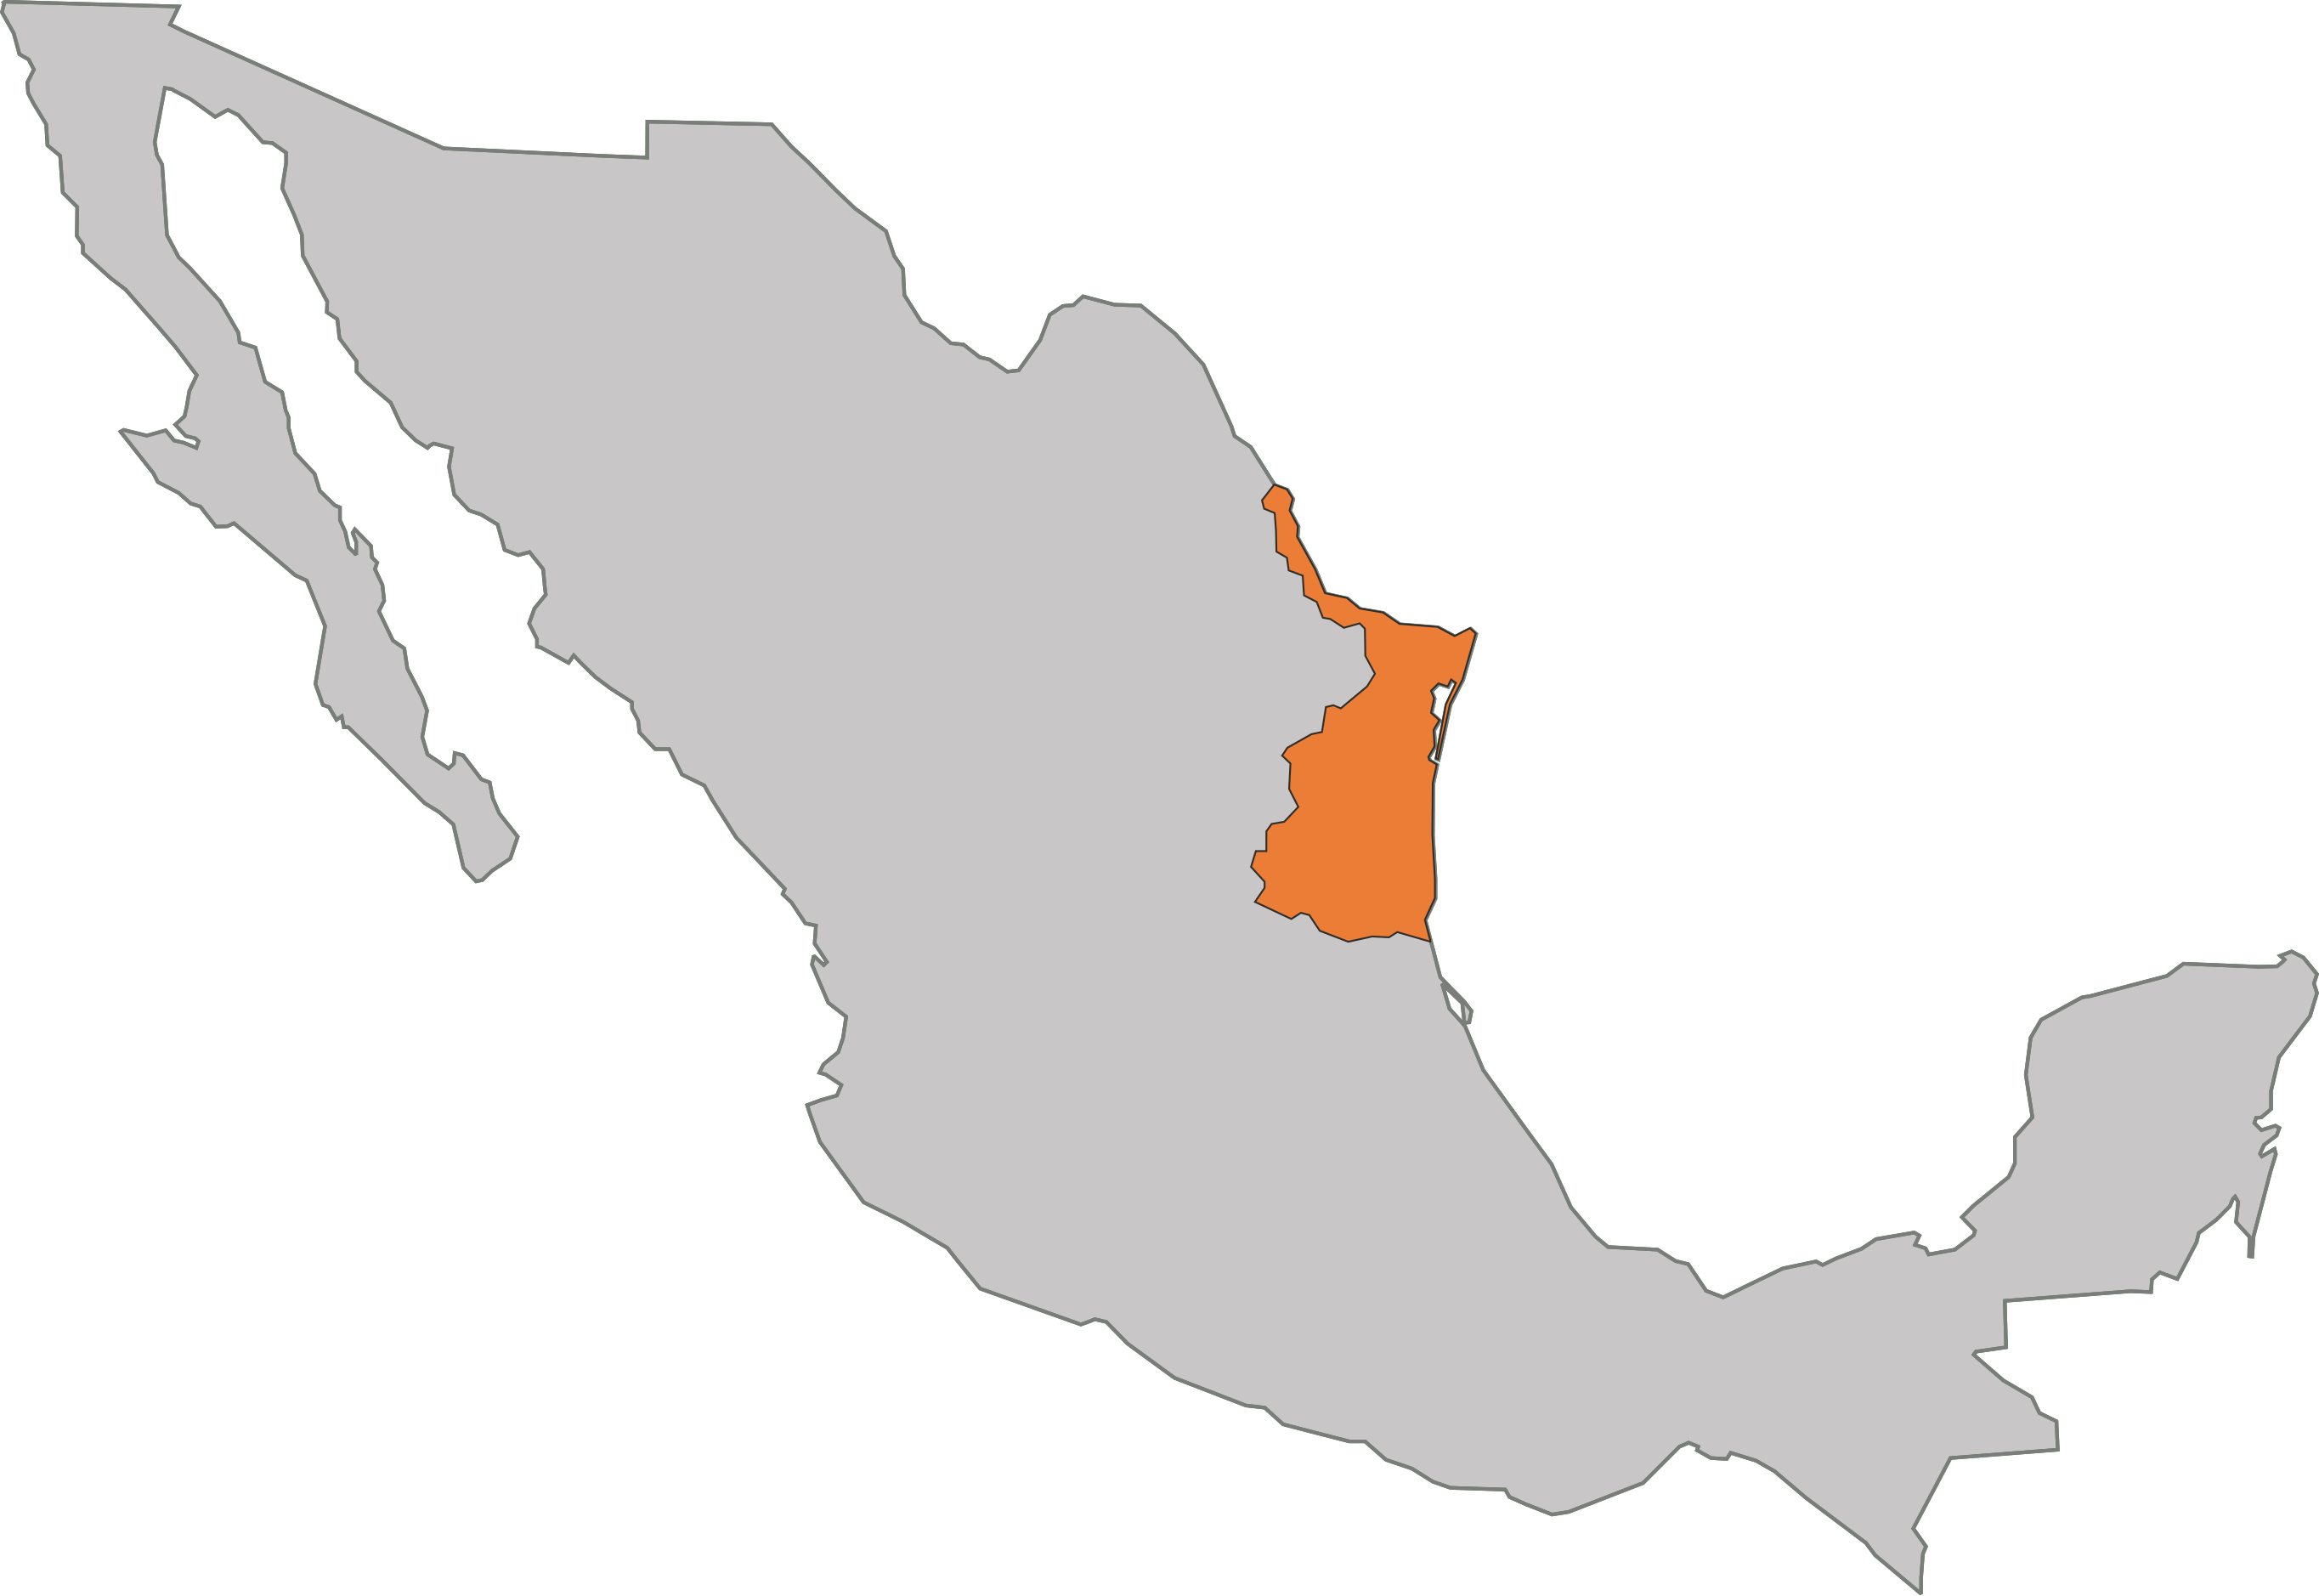
\includegraphics[width=.5\linewidth]{map}
    %\caption{Orange transportation system.}
    \label{trans}
\end{figure}

In 2011, total production was approximately 500,000 tonnes. Automatic fruit grading systems are needed to classify those quantities.

\end{frame}

\subsection{Computer vision and machine learning}
\begin{frame}
\frametitle{Computer vision and machine learning}
Computer vision is the process of understanding digital images and videos using computers. It seeks to automate tasks that human vision can achieve. This involves methods of acquiring, processing, analyzing, and understanding digital images, and extraction of data from the real world to produce information.\\

Machine learning is the study of algorithms and statistical models, which is a subset of artificial intelligence. Systems use it to perform a task without explicit instructions and instead rely on patterns and inference.

\end{frame}

\subsection{Machine learning and Decision Trees}
\begin{frame}
\frametitle{Machine learning and Decision Trees}


Decision trees (DTs) is a powerful and popular machine learning tool for classification and prediction. \\

A tree can be ``learned'' by splitting the source set into subsets based on an attribute value test. \\

Some popular algorithms for DT training are: J48, CART, ID3, C4.5 and Random Forest.

\end{frame}



\subsection{FPGA implementation advantages}
\begin{frame}
\frametitle{FPGA implementation advantages}

The most important advanges implementing an automatic fruit grading machine in a FPGA:

\begin{itemize}
 \item Reduced Power consumption
 \item Real-time responsive
 \item Industrial property protection
 \item Reduced dimension of the hardware
 \item Multiple processing lines with one device
\end{itemize}



\end{frame}

\subsection{Orange offer and demand}
\begin{frame}
\frametitle{Orange offer and demand}

\begin{figure}[h]
    \centering
    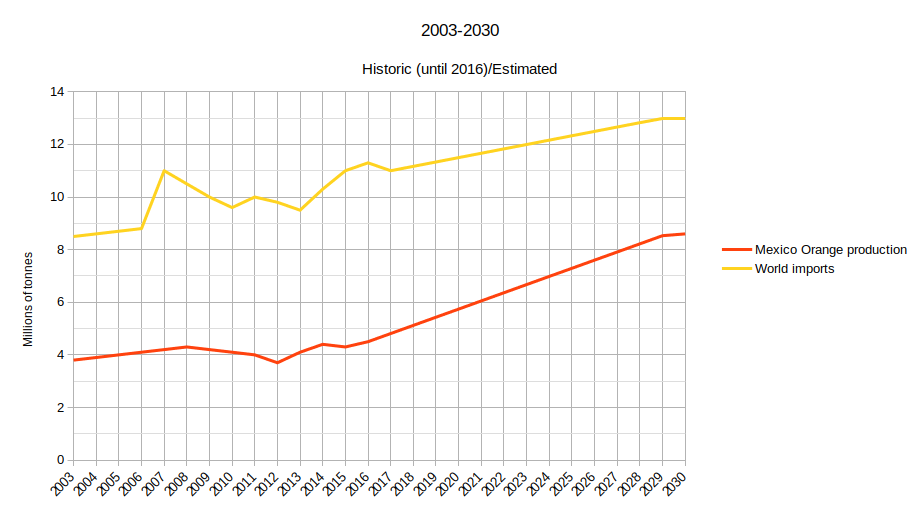
\includegraphics[width=0.9\linewidth]{grap.png}
    \label{overview}
\end{figure}

\small
International Orange consumption / Mexico Orange Production expectation.
According to Mexico's Ministry of Agriculture and Rural Development (SAGARPA).

\end{frame}





\begin{frame}
\frametitle{Planteamiento del problema}
\begin{figure}[h]
	\centering
	\begin{tabular}{ccc}
		\subfloat[Mecánica \label{lena}]{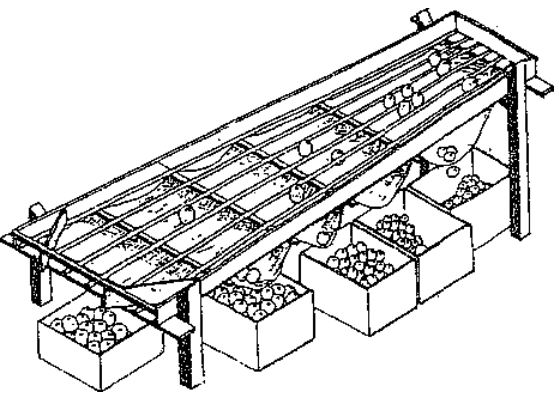
\includegraphics[width=.3\linewidth]{F/clasifMeca}} & 
		\subfloat[Manual]{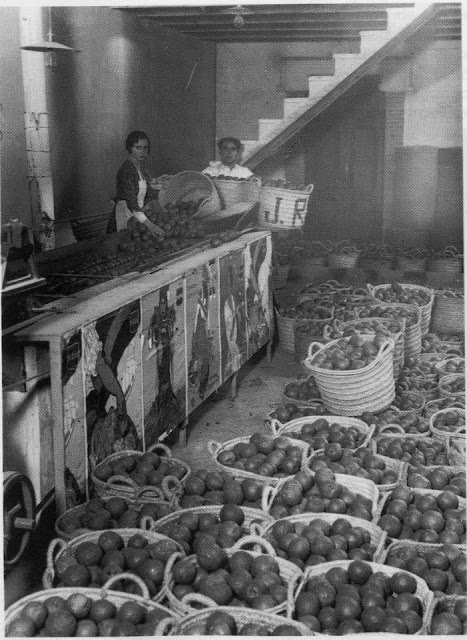
\includegraphics[width=.3\linewidth]{F/clasifMan}}  &
		\subfloat[Automática]{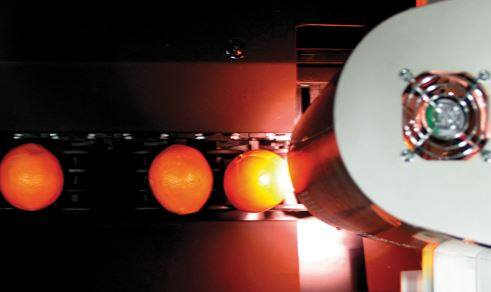
\includegraphics[width=.3\linewidth]{F/clasifAut}} 
	\end{tabular}
	
	\caption{Tipos de clasificaciones}
	\label{lumiprueb}
\end{figure}



\end{frame}

\begin{frame}
	\frametitle{Planteamiento del problema}

	Principales problemas:
	
	\begin{itemize}
		\item Manejo de empleados
		\item Sistemas informáticos obsoletos
		\item Sistemas que golpean la fruta
		\item Inconsistencia de clasificación
		\item Atascos
		\item Lentos
	\end{itemize}

	\textbf{Solución:}
	Un hardware que:
	\begin{itemize}
		\item Sea fácilmente configurable
		\item Rápido
		\item Bajo uso de recursos computacionales
	\end{itemize}
	
\end{frame}

\begin{frame}
	\frametitle{Objetivos}

	\textbf{Objetivo general}
	\begin{itemize}
		\item Desarrollar una implementación de hardware en FPGA capaz de clasificar naranjas con una precisión del 90\% con una rapidez de 1 naranja por segundo.
	\end{itemize}
	
	\textbf{Objetivos específicos}
	\begin{itemize}
		\item Implementación en FPGA de un clasificador por árbol de desición.
		\item Implementación en FPGA de un procesador de video extractor de características.
		\item Implementación de hardware  auxiliar para mejorar el tiempo de desarrollo (microcontrolador).
	\end{itemize}
\end{frame}


\section{Proposed Architecture}
\begin{frame}
\frametitle{Vista del sistema}

%The main components of the proposed system are shown. An industrial camera takes input video and transmits to FPGA using a HDMI cable. The camera is located inside a dark cabin with a rail, which provides a controlled environment (constant illumination and black background). On the rail, oranges are transported and passed in front of the camera at a speed of 4 \textbf{oranges per second} (ops).


\begin{figure}[h]
    \centering
    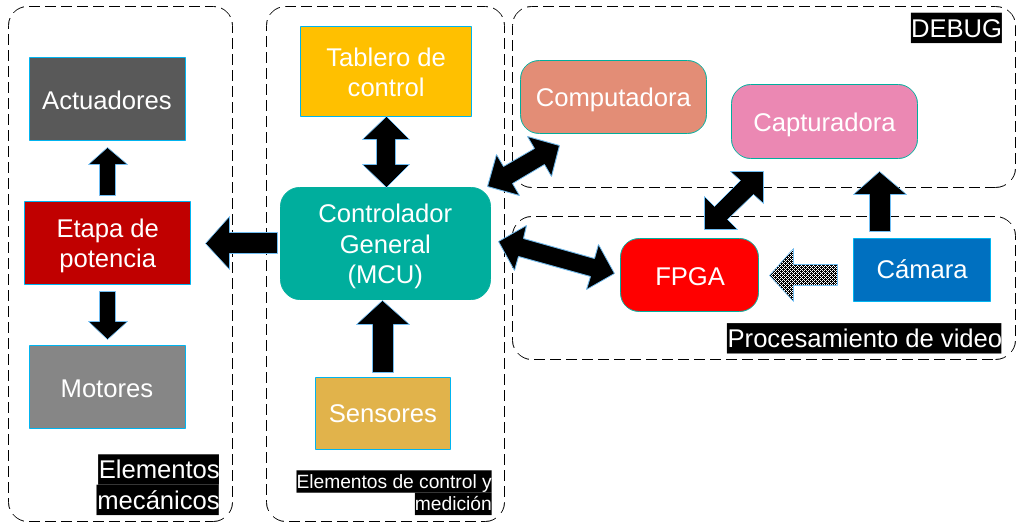
\includegraphics[width=\linewidth]{F/diagramagralelectrico}
    %\caption{System elements overview.}
    \label{overview}
\end{figure}

%FPGA: Image processor.\\
%$\mu$C: Sensor/actuator manager.\\
%Camera: video acquisition.\\
%Capturer: Debugging, measuring and testing. (Not part of the final hardware)\\
%Display: Debugging.

\end{frame}


\subsection{Project platform}
\begin{frame}
\frametitle{Project platform}
\begin{figure}[h]
    \centering
    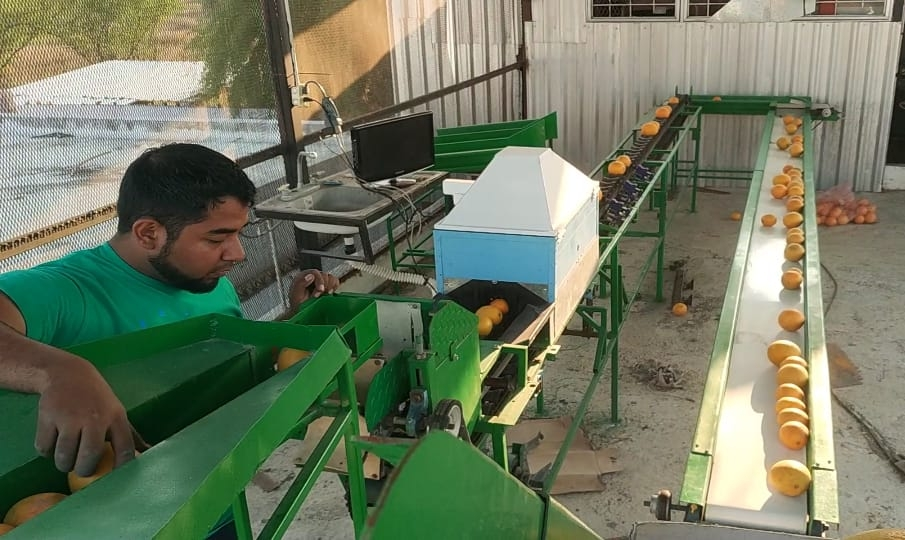
\includegraphics[width=\linewidth]{maq.jpeg}
    %\caption{Orange transportation system.}
    \label{trans}
\end{figure}
\end{frame}


\begin{frame}
	\frametitle{Project platform}
	\begin{figure}[h]
		\centering
		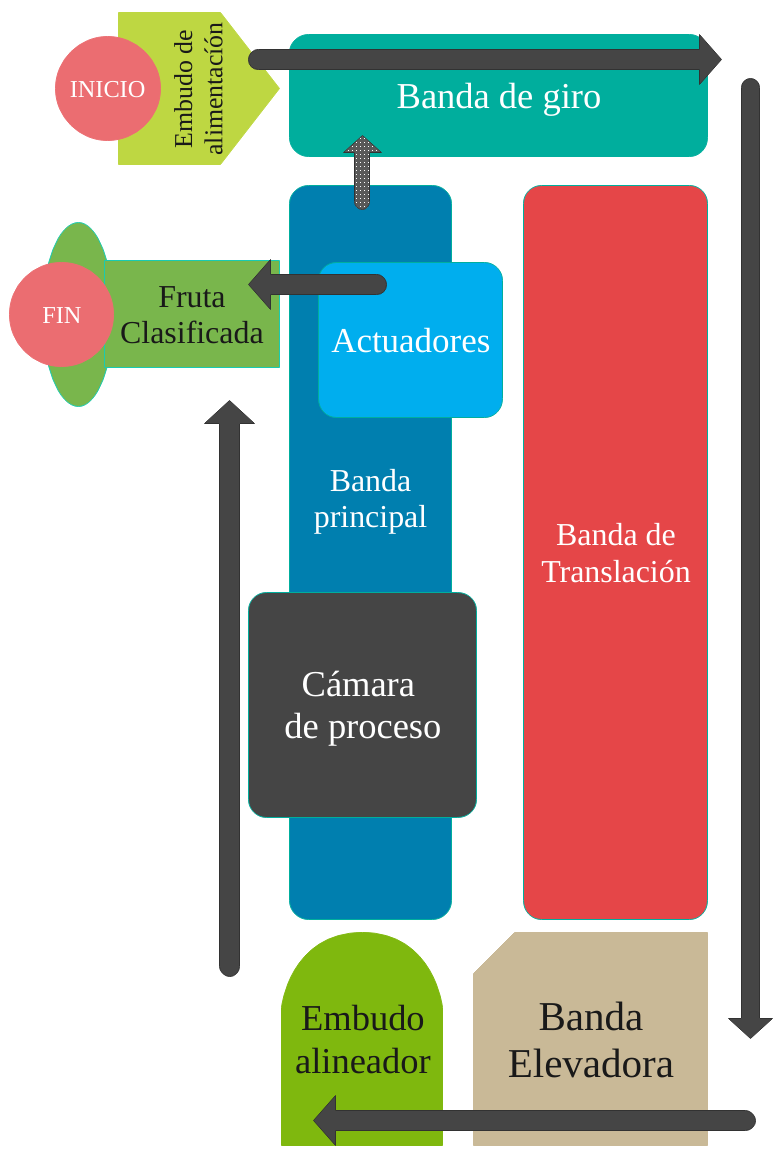
\includegraphics[width=.5\linewidth]{F/diagramamaquina}
		%\caption{Orange transportation system.}
		\label{trans}
	\end{figure}
\end{frame}

\begin{frame}
	\frametitle{Dark cabin}
	\begin{figure}[h]
		\centering
		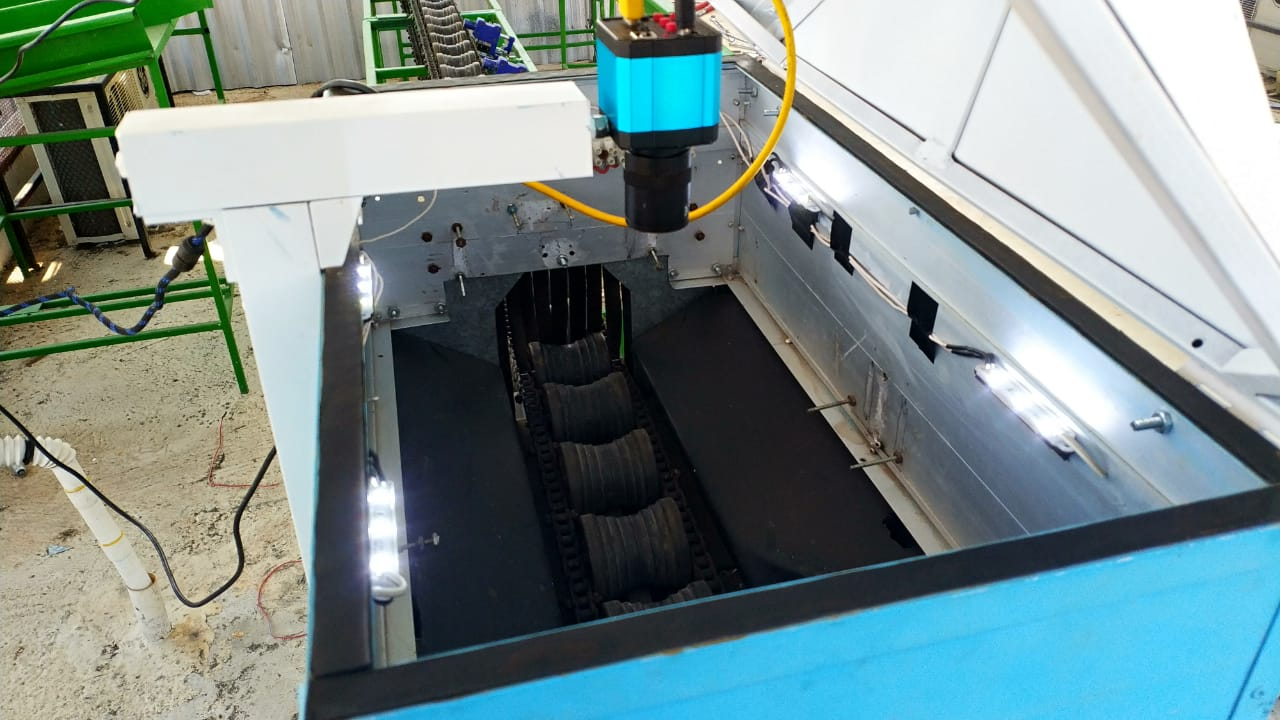
\includegraphics[width=\linewidth]{DK}
		%\caption{Dark cabin setup.}
		\label{trans}
	\end{figure}
\end{frame}

\begin{frame}
	\frametitle{Project platform}
	\begin{figure}[h]
		\centering
		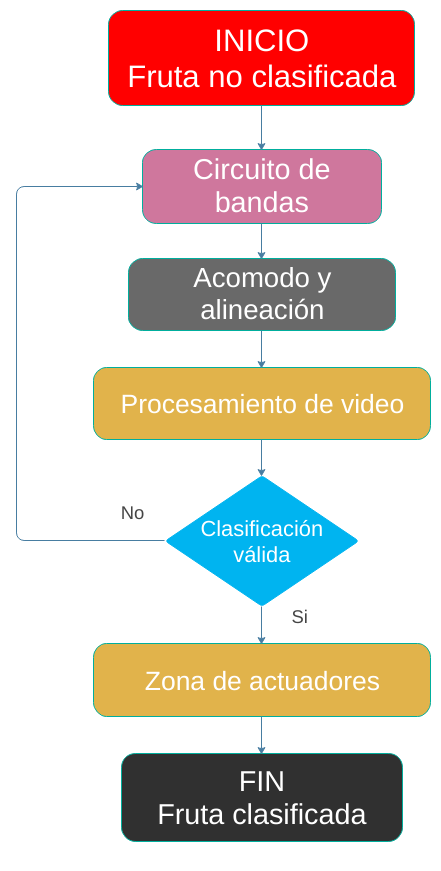
\includegraphics[width=.35\linewidth]{F/diagramaflujomaquina}
		%\caption{Orange transportation system.}
		\label{trans}
	\end{figure}
\end{frame}


\subsection{HW/SW components}
\begin{frame}
\frametitle{Hardware components}
\textbf{Resources.}

The hardware elements used for the proposed system are:
% \begin{itemize}
% \item Industrial Video Processing Kit (IVPK) Spartan6
% \item Industrial camera YW2307
% \item Atmega328
% \item HDMI display 
% \item Avermedia-C875
% \end{itemize}

\begin{figure}[h]
    \centering
    \captionsetup[subfigure]{labelformat=empty}
    \subfloat[Atmega328 $\mu$C.\label{mis}]{%
       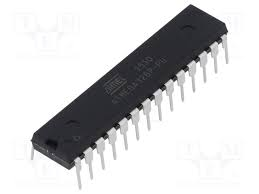
\includegraphics[width=.22\linewidth]{at}
     }
     \hfill
     \subfloat[Industrial camera YW2307.\label{oad}]{%
       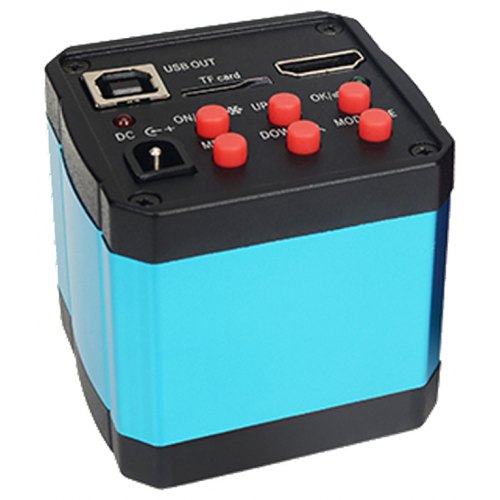
\includegraphics[width=.22\linewidth]{cam}
     }
     \hfill
     \subfloat[Avermedia-C875.\label{av}]{%
       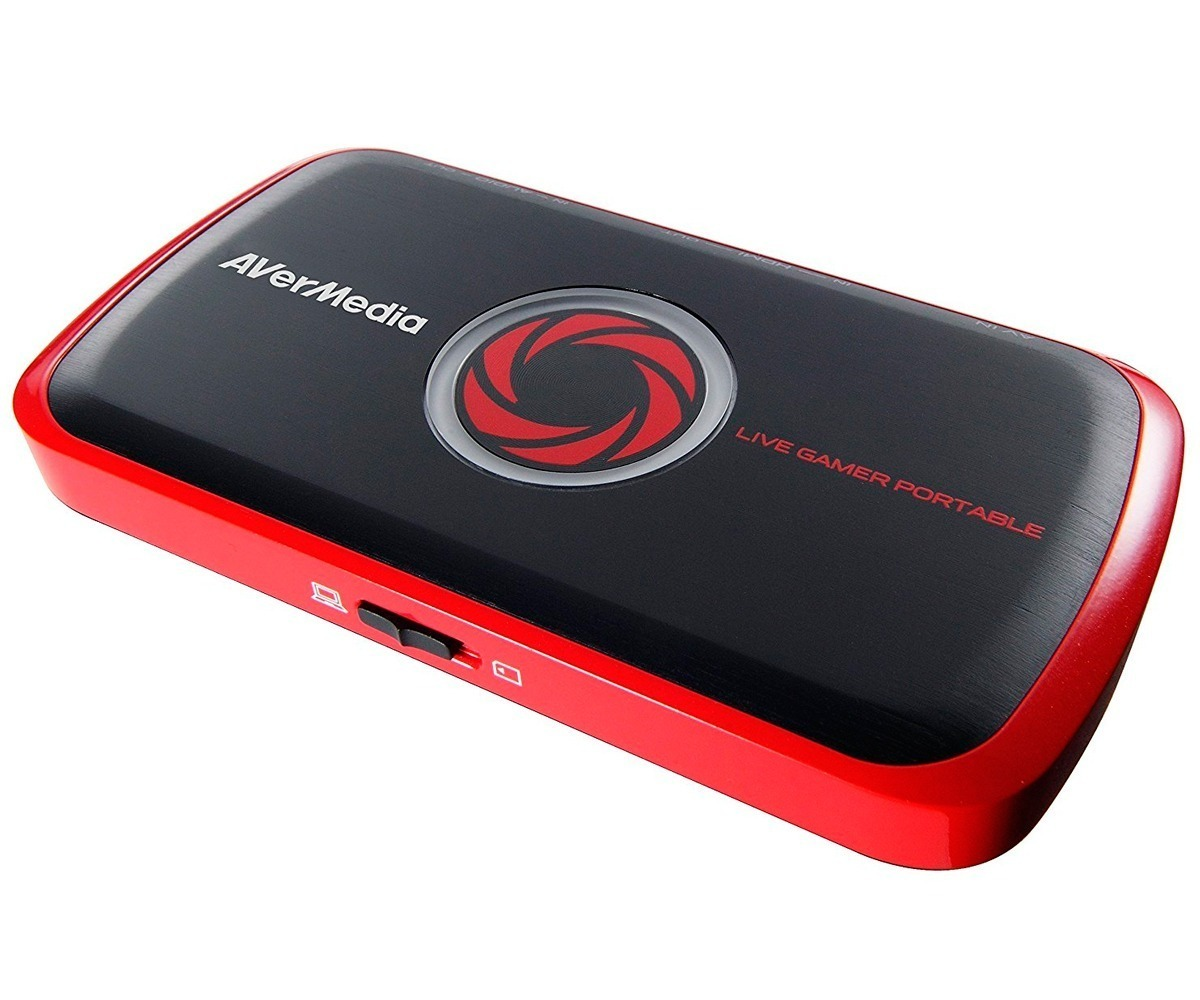
\includegraphics[width=.22\linewidth]{aver}
     }\\
     \subfloat[Industrial Video Processing Kit (IVPK) Spartan6.\label{av}]{%
       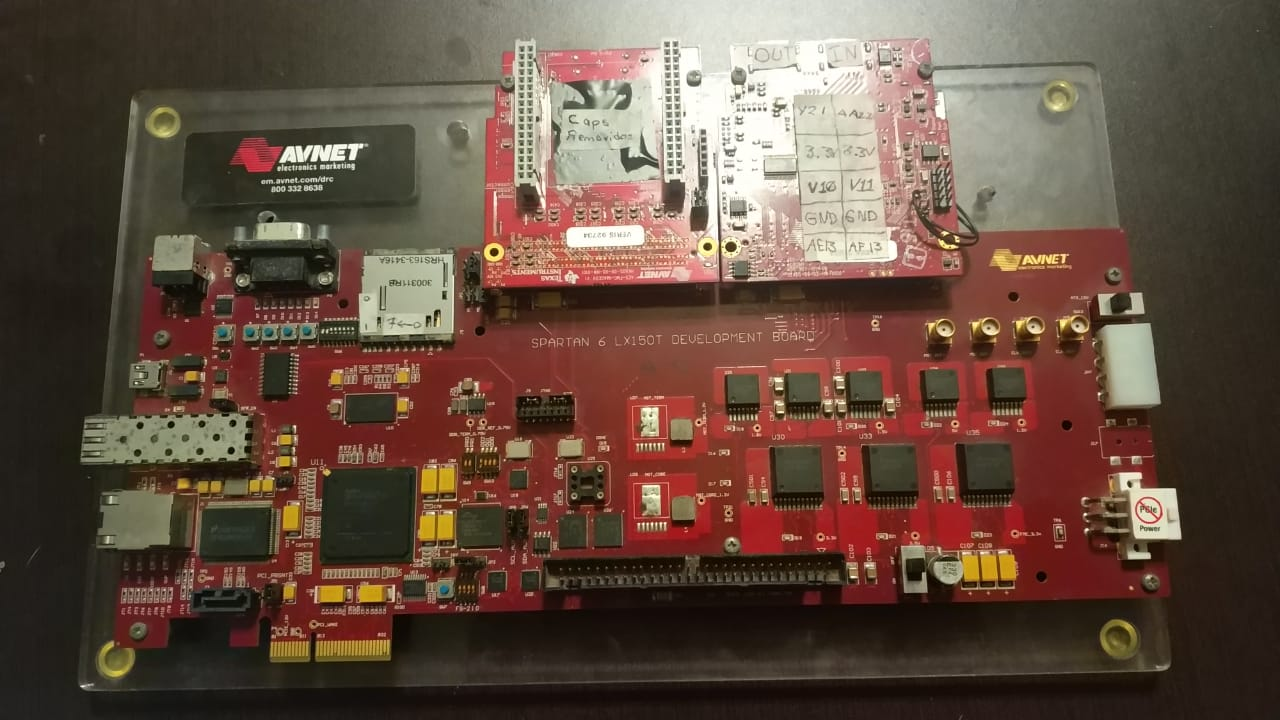
\includegraphics[width=.33\linewidth]{fpga}
     }
  
  
    %\caption{Proposed segmentation algorithm.}
    \label{segalgs}
    \end{figure}


\end{frame}



\begin{frame}
\frametitle{Software components}
\textbf{Resources.}

The software used for the proposed system are:
\begin{itemize}
\item Weka(v3): used for feature analysis and model generator.
\item Python(v3.6): used for text parsing, and feature analysis.
\item OpenCV(v4): used for image processing and data acquisition.
\item Xilinx ISE (v14.7): used for HDL synthesis and hardware debugging. 
\item Vivado (v2019.2): used for HDL synthesis and hardware debugging. 
\end{itemize}

\end{frame}


\subsection{Project methodology}
\begin{frame}
\frametitle{Project methodology}
To preform this project the following methodology was implemented:

\begin{enumerate} [a)]
 \item Decision Tree model Build (PC stage)
 \begin{enumerate}
 \item Data set acquisition (Orange images from machine platform runtime)
 \item Segmentation
  \item Feature extraction (R, G, B, H, S, V, Gray)
  \item Data set acquisition (Pixels)
  \item Feature relevance analisys
  \item Model generation (Training and Testing)
 \end{enumerate}

 \item Hardware modules (FPGA stage)
 \begin{enumerate}
  \item Pixel buffer
  \item HSV conversion
  \item Grayscale conversion
  \item DT based segmentation
  \item Morphological operations
  \item Mask drawer
 \end{enumerate}
 
 \item Integration
 \begin{enumerate}
  \item FPGA segmentation recording (Capturer)
  \item Segmentation comparison and measurements
 \end{enumerate}

\end{enumerate}
\end{frame}



\subsection{Data set acquisition procedure}
\begin{frame}
\frametitle{Data set acquisition procedure}
\begin{enumerate}
 \item Record video
 \item Region of interest (ROI) cropping
 \item OpenCV segmentation
 \item Center detection
 \item Automated orange image acquisition
 \item Manual image classification
 \item Feature extraction (HSV and Grayscale conversion)
 \item Pixel data set acquisition (Segmentation vs Features)
\end{enumerate}
\end{frame}

\begin{frame}
\frametitle{Data set acquisition (Orange images)}
    \begin{figure}[h]
    \centering
    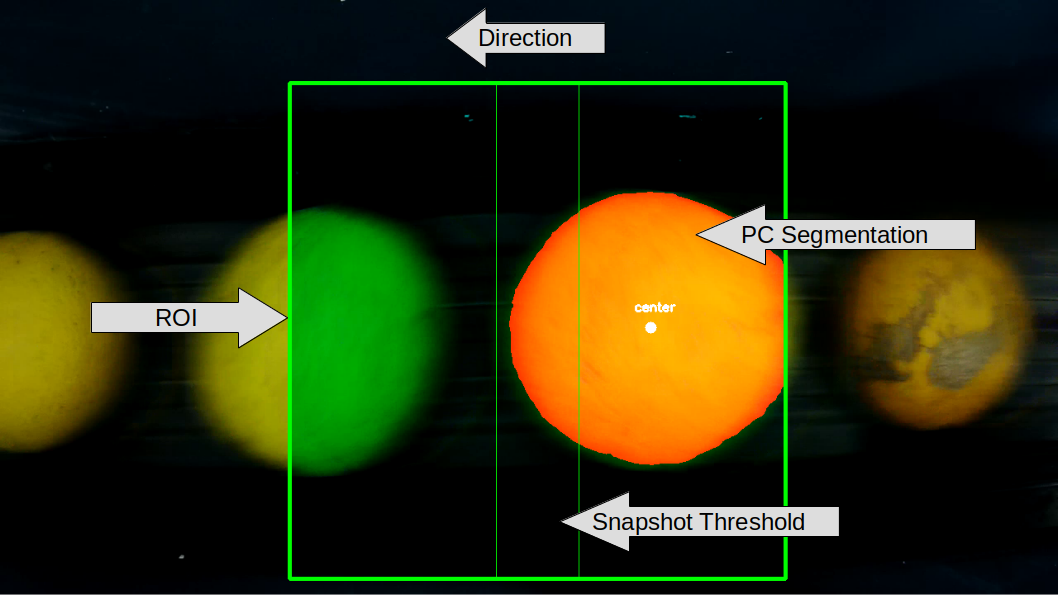
\includegraphics[width=\linewidth]{framito2.png}  
    %\caption{Video frame processing.}
    \label{vaf}
    \end{figure}
\end{frame}


\begin{frame}
\frametitle{Data set acquisition (Pixels)}

Feature extraction from every channel from RGB, HSV, and Grayscale color spaces.
%Once the images of oranges were properly classified  by size and color each image is converted to HSV and Grayscale color spaces for taking the 7 features and build the DT model.\\

%The data set is compiled with the 7 feature and the pixel in segmentation as class (segmented pixel / non-segmented pixel).

\begin{figure}[h]
        \centering
        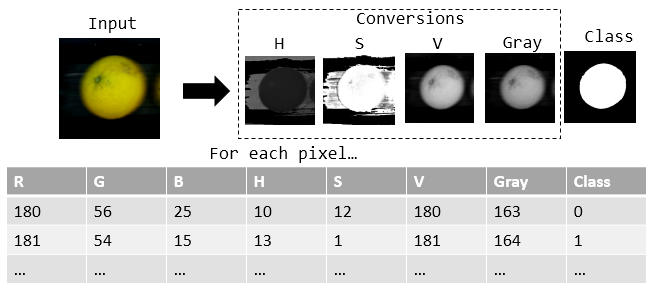
\includegraphics[width=\linewidth]{ftEx}  
        %\caption{Feature extraction schema.}
        \label{ftex}
    \end{figure}

\end{frame}

\begin{frame}
	\frametitle{Adquisición Data set de color}
	
	%Once the images of oranges were properly classified  by size and color each image is converted to HSV and Grayscale color spaces for taking the 7 features and build the DT model.\\
	
	%The data set is compiled with the 7 feature and the pixel in segmentation as class (segmented pixel / non-segmented pixel).
	
	\begin{figure}[h]
		\centering
		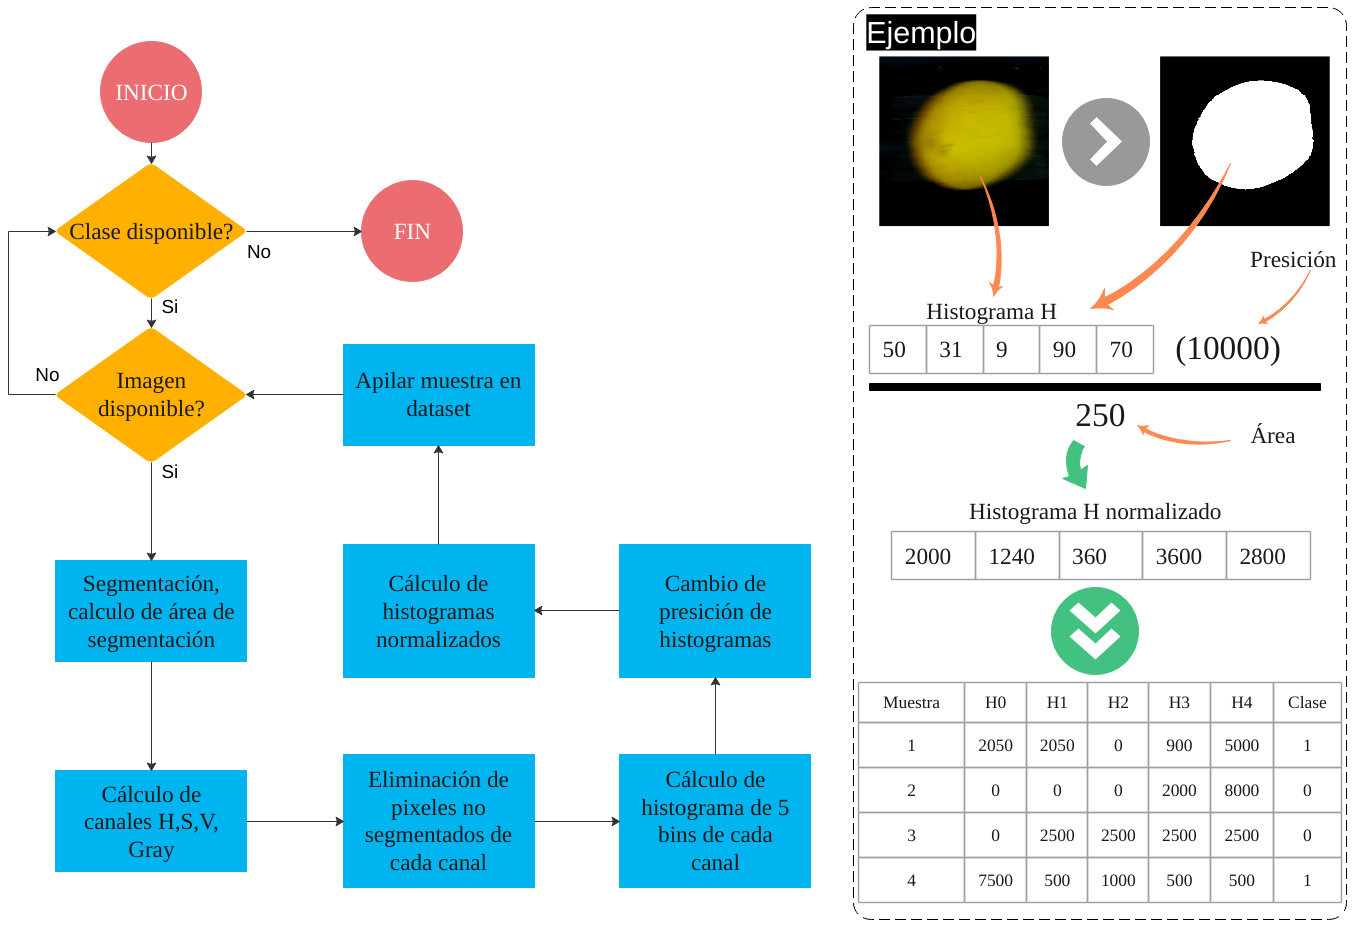
\includegraphics[width=\linewidth]{F/dscolor}  
		%\caption{Feature extraction schema.}
		\label{ftex}
	\end{figure}
	
\end{frame}



\begin{frame}
	\frametitle{Model generation}
	
	\begin{figure}[h]
		\centering
		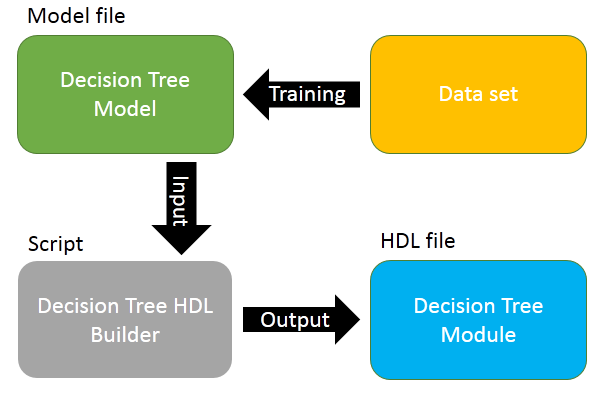
\includegraphics[width=0.7\linewidth]{weka_overview.png}  
		%\caption{Decision Tree module generator.}
		\label{weki}
	\end{figure}
\end{frame}




%\subsection{Feature relevance analisys}
\begin{frame}
\frametitle{Feature relevance analisys}
A feature analysis to obtain the best features for building the model was performed. The following analysis were used:
\begin{enumerate}
    \item Relative Absolute Error (RCA).
    \item Correlation Attribute analysis (CAA).
    \item Info Gain Attribute Evaluation (IGAE).
    \item Gini impurity (GI)
    \item Entropy (E)
\end{enumerate}
\end{frame}





% \begin{frame}
% \frametitle{Hardware overview}
% The proposed hardware modules are depicted the following picture. The input of the main module are the 24 bits of the $RGB$ frames and the video synchronization signals: video clock, hsync, and vsync. On the other hand, the outputs are the same synchronization signals and the 24 processed bits of RGB. All input signals are generated by the camera and connected through an HDMI port, as well as the output signals.
% 
% \end{frame}



% \begin{frame}
% \frametitle{Module description}
% \begin{itemize}
%     \item \textbf{Pixel buffer module}\\
%     This module handles $RGB$ bus and synchronization signals. All synchronization signals are buffered in this stage to prevent signal deformation. $RGB$ bus is stored in a register to be able to read by any other modules.\\
% 
%     
%     \item \textbf{HSV conversion module}\\
%     This module makes a conversion from $RGB$ to HSV color space and is based on the OpenCV documentation. It is a combinational circuit that calculates each components.
%     
%     \item \textbf{Gray scale conversion module}\\
%     As mentioned in a previous section, to calculate gray-scale pixel was used equation \ref{eqLuma}. Fixed point arithmetic was used to calculate the output.\\
% \end{itemize}
% \end{frame}


%\begin{frame}
%\frametitle{Module description}
%\textbf{Morphological operations module (MOM)}\\
%%     This module receives the segmented frame as input. Its main purpose is to eliminate porosity and noise in the segmented object. It consist in a Closing + Dilation morphological operations applied in series. Closing operation was performed using a $7 \times 7$ disk structuring element. Dilation was applied using a $3 \times 3$ disk structuring element. This module shifts segmentation 10 vertical and horizontal pixels (4 pixel for each $7\times7$ kernel and 2 more for $3\times3$ kernel). Clock video signal is needed to synchronize the register where the segmentation is stored.\\
%
%       \begin{figure}[h]
%    \centering
%    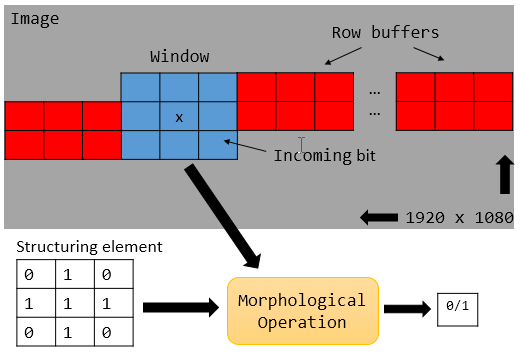
\includegraphics[width=0.8\linewidth]{mom}
%    %\caption{Morphological Operations Module (MOM) behavior.}
%    \label{modules}
%\end{figure} 
%\end{frame}

%\begin{frame}
%\frametitle{Module description}
%    
%\textbf{Mask drawer module}\\
%%     Once the segmentation is done, the border of the segmented structure is drawn in cyan color over the input frame. This can be done by the multiplexers. When the module finds a segmented pixel, it prints a cyan pixel, otherwise prints the value of the input pixel.
%%     The purpose of marking these border pixels is to make easier for the FPGA to segment the structure and to synchronize videos to make an I/O video comparison.
%
%    \begin{figure}[h]
%    \centering
%    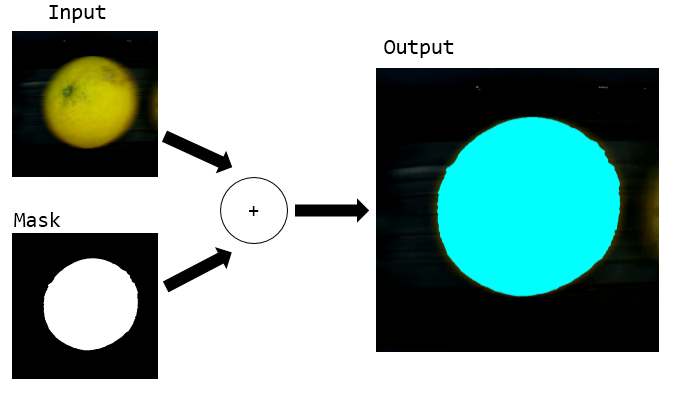
\includegraphics[width=\linewidth]{mkdwsch}
%    %\caption{Mask drawer behavior.}
%    \label{modules}
%\end{figure}
%
%\end{frame}


\begin{frame}
\frametitle{Segmentation module}
    
    The module was generated with Decision Tree HDL Builder script (SCHADD). The algorithm only can solve decision trees with binary nodes, also the output only can be binary (only can be classified 2 classes).\\ 
    
    This approach has the following advantages:\\
    
    \begin{itemize}
    
    \item Reducing and mantaining the combinational path to be the same in all of its parts.
    
    \item Tree depth to be less significative, since it only needs more comparators.\\
    
    \end{itemize}

    
\end{frame}

\begin{frame}
\frametitle{Decision Tree (DT)}
\begin{figure}[h]
    \centering
    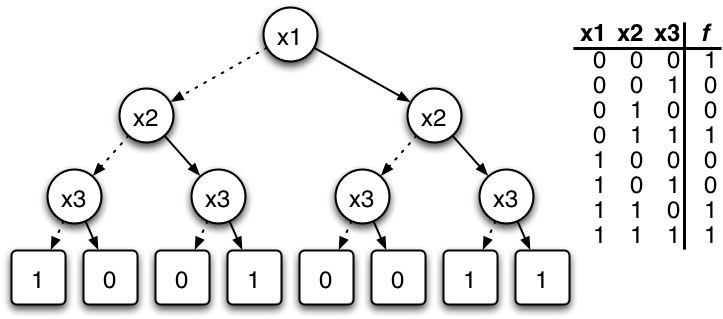
\includegraphics[width=0.8\linewidth]{BDD.png}
    %\caption{Binary Decision Tree Example.}
    \label{overview}
\end{figure}

\small
\begin{itemize}
 \item Easy hardware implementation (only uses comparators).
 \item No complex arithmetic operations.
 \item No resource expensive.
 \item Can be solved as a parallel circuit (equal combinational path).
\end{itemize}


\end{frame}


\begin{frame}
	\frametitle{Model generation}
	
	\begin{figure}[h]
		\centering
		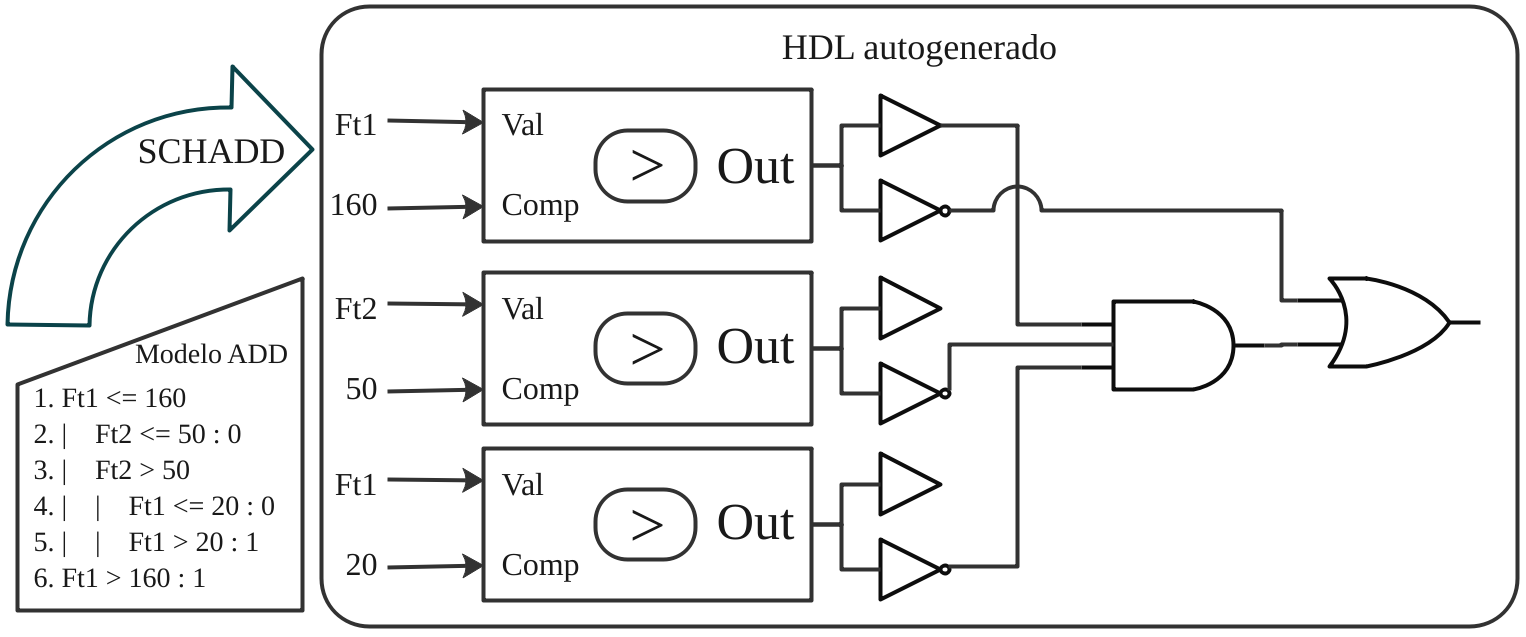
\includegraphics[width=0.9\linewidth]{F/addex}  
		%\caption{Decision Tree module generator.}
		\label{weki}
	\end{figure}
	
	SCHADD: Script Constructor HDL de Arbol de Desición
	
\end{frame}

\begin{frame}
	\frametitle{Arquitectura general}
	
	\begin{figure}[h]
		\centering
		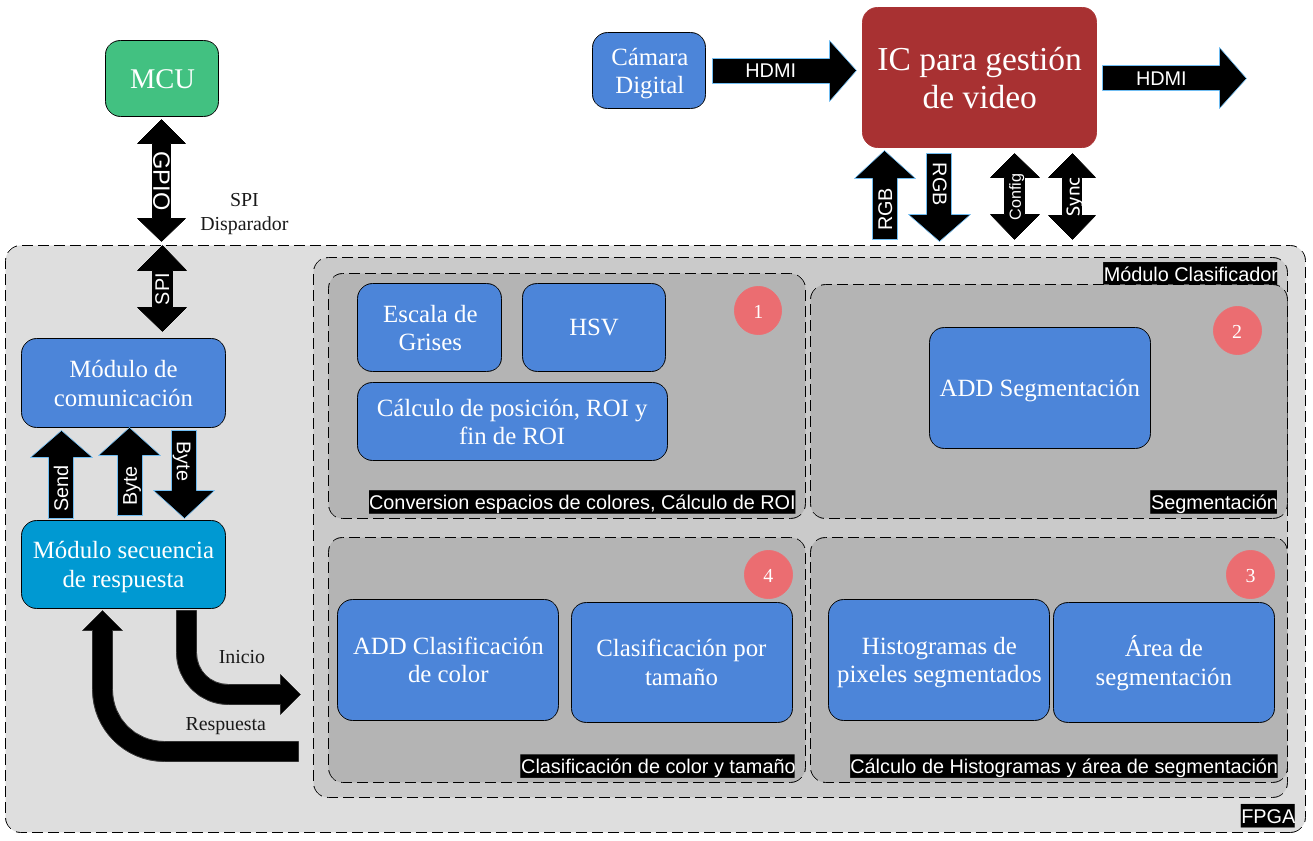
\includegraphics[width=0.9\linewidth]{F/arquitectura}  
		%\caption{Decision Tree module generator.}
		\label{weki}
	\end{figure}
	
	
\end{frame}



\section{Results}

\begin{frame}
\frametitle{Results}
\textbf{Data sets acquired}

\begin{table}[h]
\centering
%\resizebox{\linewidth}{!}{%
%\caption{Generated data set details.}
    \begin{tabular}{|c|c|c|}
    \hline
    Resource & N. samples & Description\\
        \hline
    Video  & 3 & Low speed (0.5 ops) (720p,60fps)\\
        \hline
    Video  & 3 & Medium speed (2 ops) (720p,60fps)\\
        \hline
    Video  & 3 & High speed (5 ops) (720p,60fps)\\
        \hline
    Images & 1836 & Oranges photos (600x600)\\
        \hline
    Images & 1836 & Segmented Oranges photos (600x600)\\
        \hline
    Pixels & 136886 & Pixel samples (7 features, 2 classes)\\
        \hline
    \end{tabular}
    %}
    
    \label{dst}
\end{table}

Videos were recorded with different speeds (measured in oranges per second or \textbf{ops}) on platform machine runtime. Images taken from videos automatically by script. Pixels taken by every image (duplicated pixels removed).


\end{frame}



%\begin{frame}
%\frametitle{Thresholding algorithm comparison}
%%\textbf{Thresholding algorithm comparison}
%\begin{figure}[h]
%    \centering
%    \captionsetup[subfigure]{labelformat=empty}
%    \subfloat[Manual image segmentation.\label{mis}]{%
%       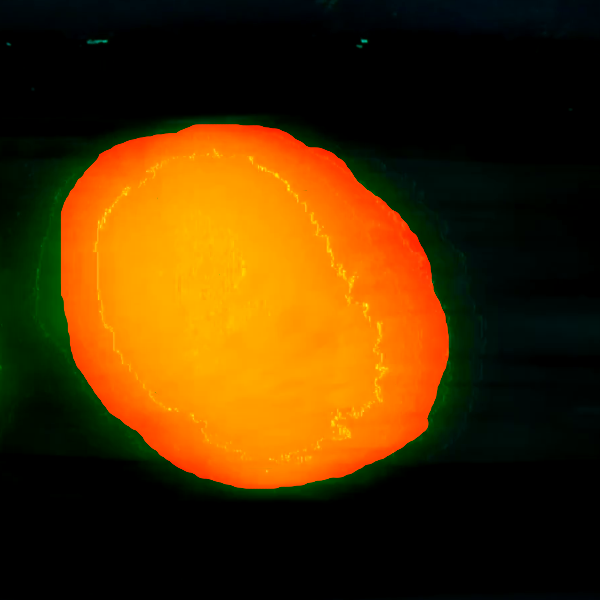
\includegraphics[width=.3\linewidth]{sgmdiff/origman.png}
%     }
%     \hfill
%     \subfloat[Otsu adaptive thresholding result. (PC)\label{oad}]{%
%       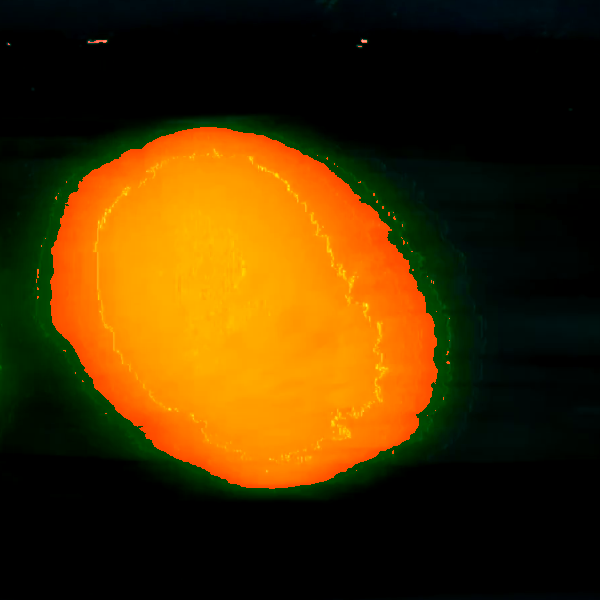
\includegraphics[width=.3\linewidth]{sgmdiff/oriot.png}
%     }
%     \hfill
%     \subfloat[Proposed segmentation. (PC)\label{purs}]{%
%       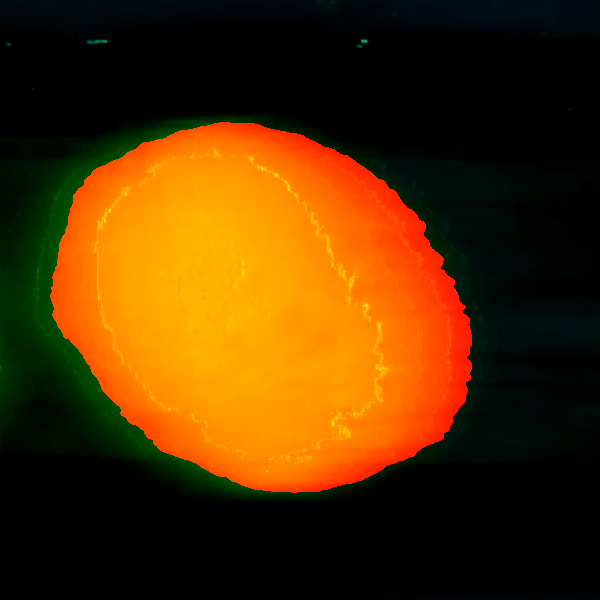
\includegraphics[width=.3\linewidth]{sgmdiff/orimk.png}
%     }
%  
%    %\caption{Proposed segmentation algorithm.}
%    \label{segalgs}
%    \end{figure}
%    
%      The resulting accuracy was 96.6\% for
%the Otsu algorithm and 97.3\% for the proposed one. Proposed algorithm only takes the biggest segmented area.
%\end{frame}



\begin{frame}
 \frametitle{Feature relevance analysis}
 \begin{table}[h]
\centering
  \caption*{FEATURE RELEVANCE ANALYSIS}
\resizebox{\linewidth}{!}{%
    \begin{tabular}{|c|c|c|c|c|c|c|c|}
    \hline
    Analysys/feature & R & G & B & H & S & V & Gray\\
        \hline
    RAE & 0.0255 & \textbf{0.0194} & 0.0195 & 0.226 & 0.0262 & 0.0166 & \textbf{0.0143}\\
        \hline
    CCA & 0.3211 & \textbf{0.5164} & 0.113 & 0.2362 & 0.0489 & \textbf{0.4733} & 0.4652\\
        \hline
    IGAE & 0.1363 & \textbf{0.2596} & 0.0696 & 0.2004 & 0.1210 & 0.2311 & \textbf{0.2370}\\
        \hline
	GI & 0.1211 & \textbf{0.2031} & 0.1024 & 0.1552 & 0.1111 & 0.1387 & \textbf{0.1681} \\ 
		\hline
	E & 0.1235 & \textbf{0.1909} & 0.1144 & 0.1598 & 0.1167 & 0.1332 & \textbf{0.1611} \\         
		\hline
    \end{tabular}}
  
    \label{importances}
\end{table}

Values shown in bold are the top 2 best values. The result shows G and Gray channels are the best features.
\end{frame}


\begin{frame}
 \frametitle{DT model training}
 \begin{table}[h]
\caption*{TREE MODEL DETAILS}
%\resizebox{\linewidth}{!}{%
    \begin{tabular}{|c|c|c|c|}
    \hline
    Model & Features  & Validation type & \begin{tabular}{c}
         Validation  \\
         accuracy
    \end{tabular}\\
    \hline
    M0 & Gray \& Hue  &
    \begin{tabular}{c}
         10-fold  \\
         70\%-Test 30\%-Train 
    \end{tabular}
    & 
    \begin{tabular}{c}
         83.24\%\\
         83.17\%
    \end{tabular}\\
        \hline
    M2 & Gray \& Green  &
    \begin{tabular}{c}
         10-fold  \\
         70\%-Test 30\%-Train 
    \end{tabular}
    & 
    \begin{tabular}{c}
         81.67\%\\
         81.50\%
    \end{tabular}\\
        \hline
    M4 & All &
    \begin{tabular}{c}
         10-fold  \\
         70\%-Test 30\%-Train 
    \end{tabular}
    & 
    \begin{tabular}{c}
         \textbf{83.52\%}\\
         \textbf{83.41\%}
    \end{tabular}\\
        \hline
    \end{tabular}
    %}
    \label{wekaacc}
\end{table}

Models tested with different feature combination.  $MO$ was considered the best since H channel is good for color segmentation. The training results show the best model is $M4$    .

\end{frame}



\begin{frame}
\frametitle{Decision Tree models}
\begin{table}[h]
\caption*{MODEL SEGMENTATION DESCRIPTIONS.}
\centering
%\resizebox{\linewidth}{!}
    \label{modelsdetails}
\end{table}

Only odd number models have Morphologic operations, to get a better segmentation performance. 

\end{frame}


\begin{frame}
\frametitle{FPGA+DT model segmentation result}

    \begin{figure}[h]
    \captionsetup[subfigure]{labelformat=empty}
    \centering
    \subfloat[Sample frame.\label{nf}]{%
       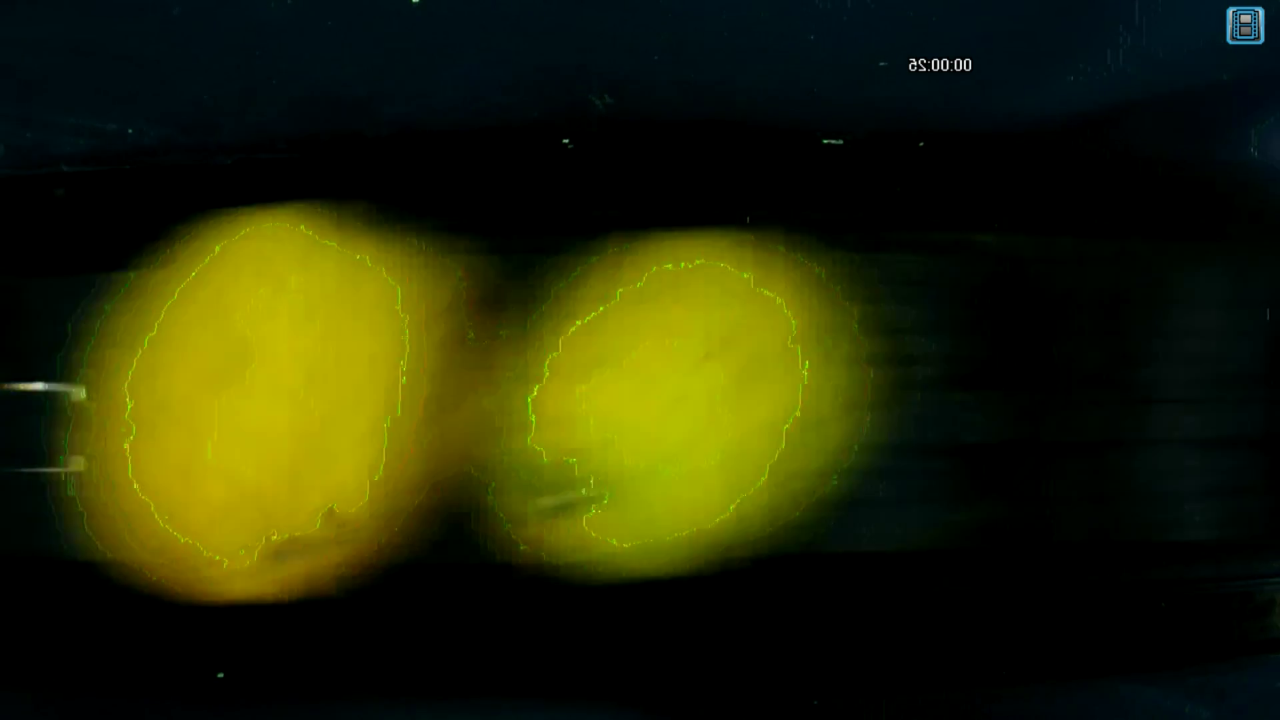
\includegraphics[width=.3\linewidth]{segmented/m31_orig.png}
     }
     \\
     \subfloat[$M0$ segmentation.\label{M0seg}]{%
       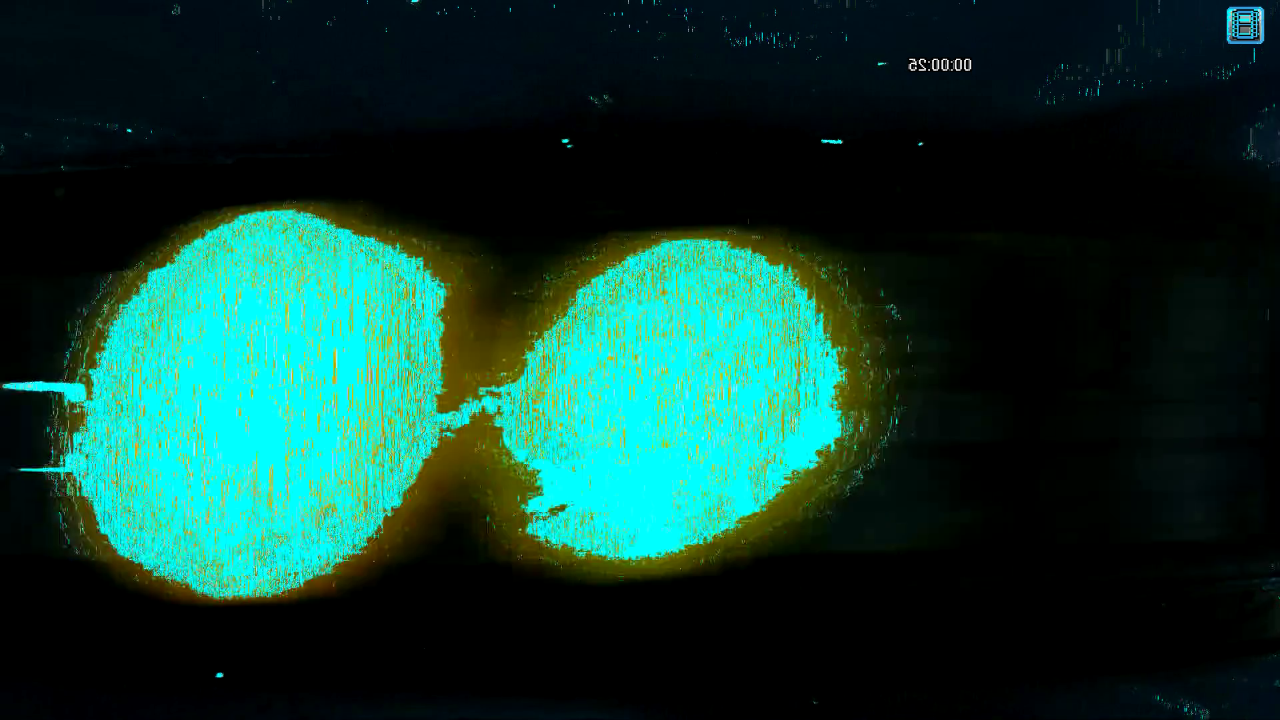
\includegraphics[width=.3\linewidth]{segmented/M0_m31_processed.png}
     }
     \hfill
     \subfloat[$M1$ segmentation.\label{M1seg}]{%
       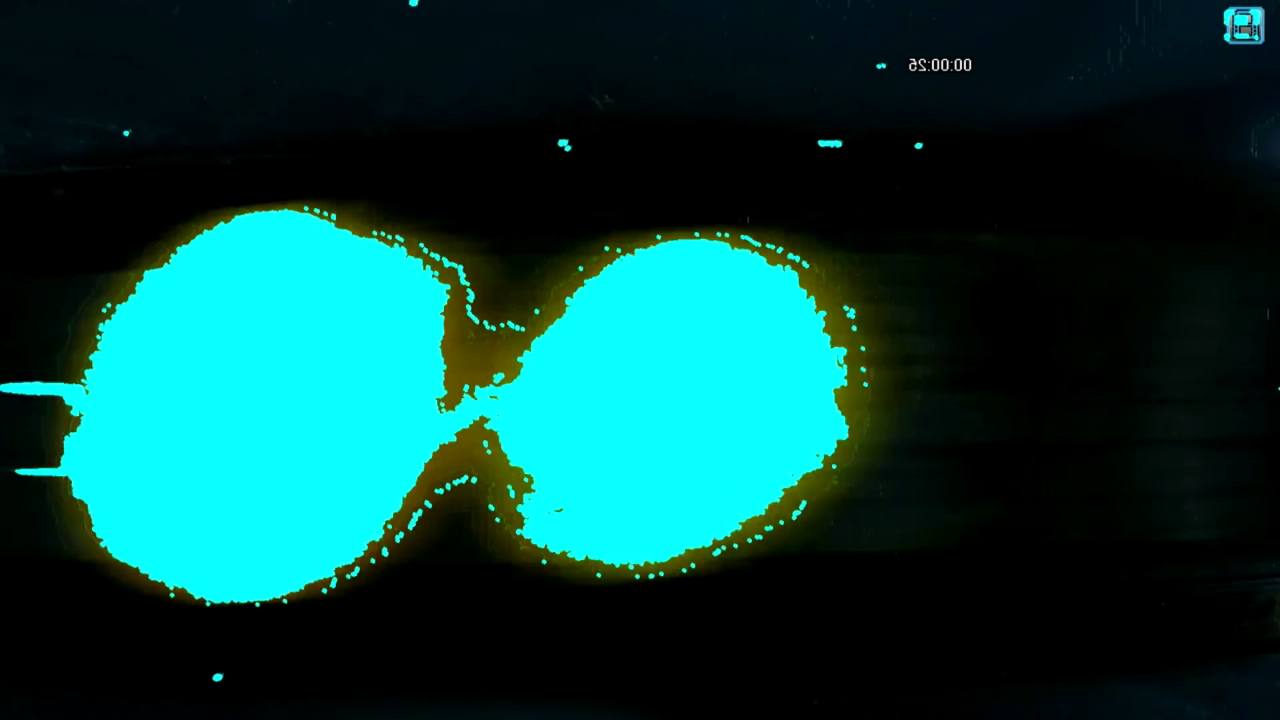
\includegraphics[width=.3\linewidth]{segmented/M1_m31_processed.png}
     }
     \hfill
     \subfloat[$M2$ segmentation.\label{M2seg}]{%
       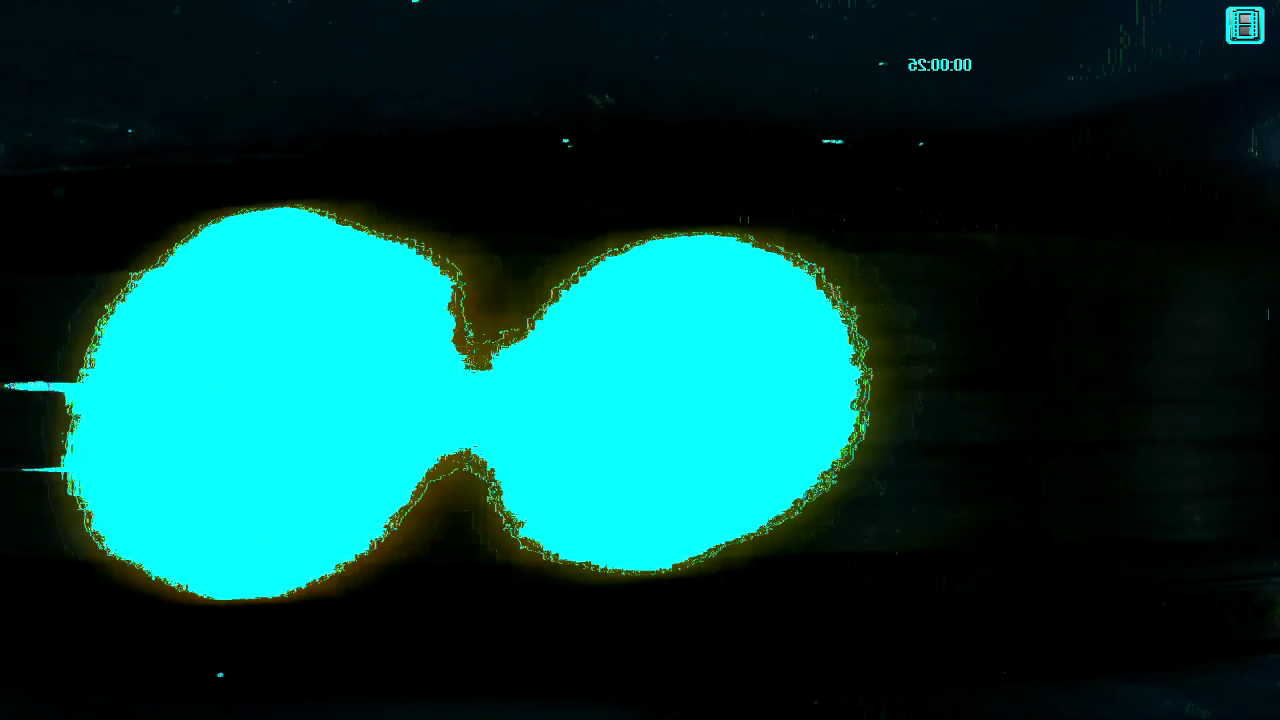
\includegraphics[width=.3\linewidth]{segmented/M2_m31_processed.png}
     }
     \\
     \subfloat[$M3$ segmentation.\label{M3seg}]{%
       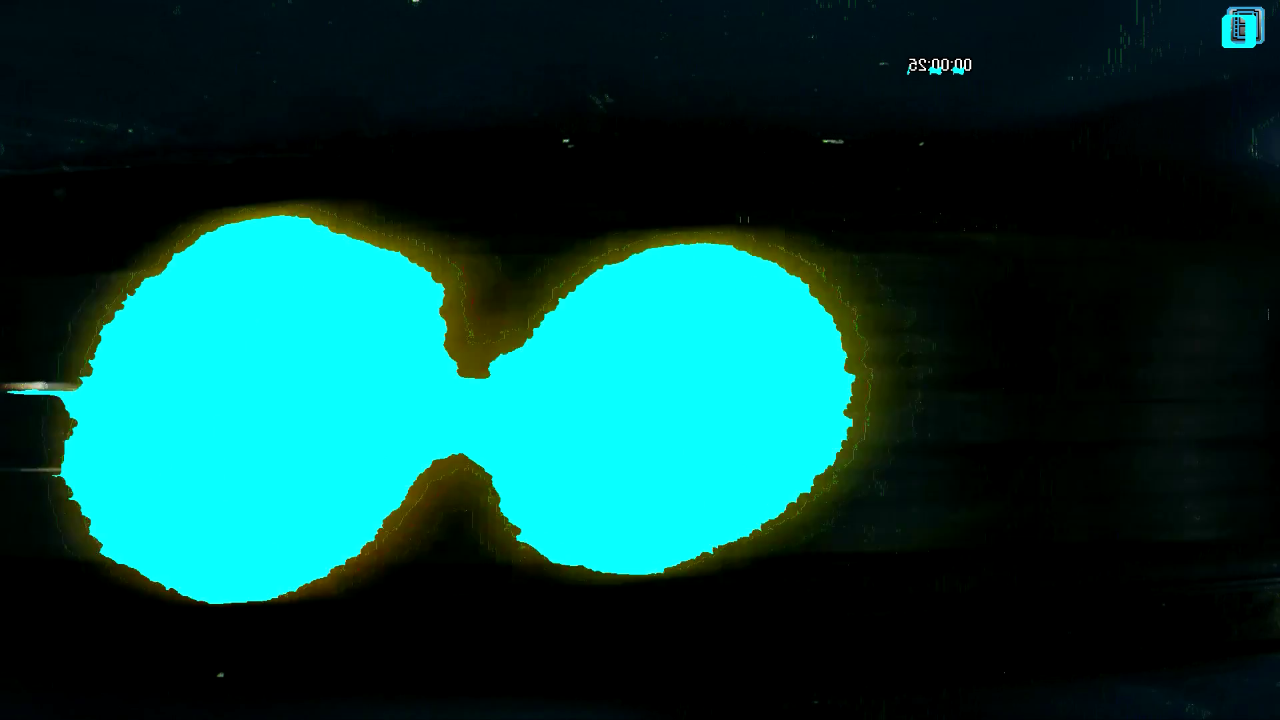
\includegraphics[width=.3\linewidth]{segmented/M3_m31_processed.png}
     }
     \hfill
     \subfloat[$M4$ segmentation.\label{M4seg}]{%
       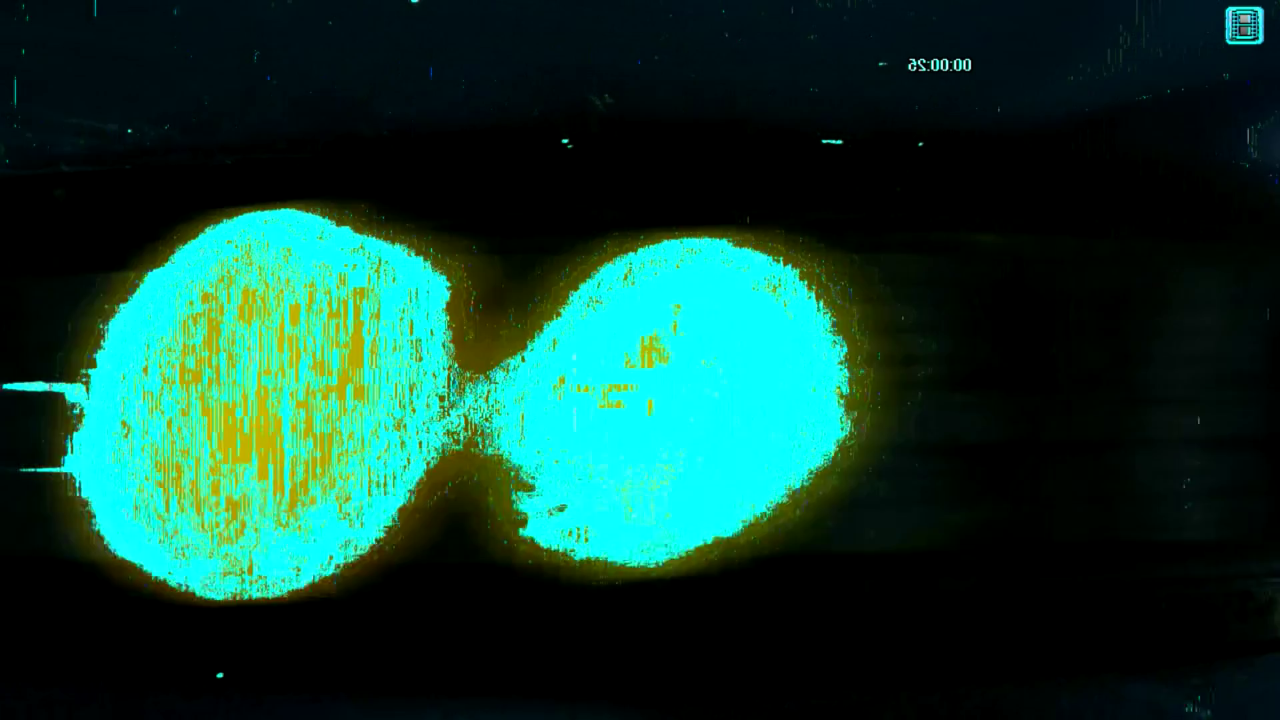
\includegraphics[width=.3\linewidth]{segmented/M4_m31_processed.png}
     }
     \hfill
     \subfloat[$M5$ segmentation.\label{M5seg}]{%
       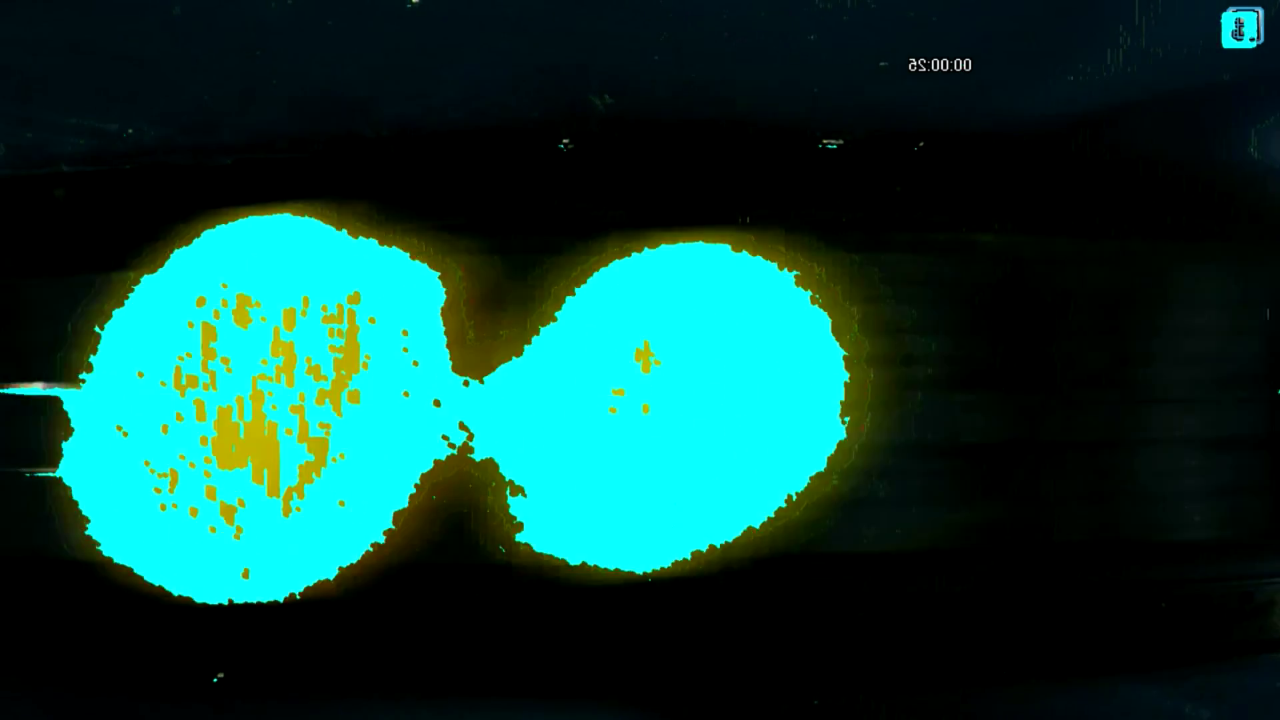
\includegraphics[width=.3\linewidth]{segmented/M5_m31_processed.png}
     }

    \caption{Different outputs of the segmentation models.}
    \label{segouts}
    \end{figure}
\end{frame}


\begin{frame}
\frametitle{Thresholding algorithm comparison}
\begin{figure}[h]
    \centering
    \captionsetup[subfigure]{labelformat=empty}
    \subfloat[PC segmentation\label{oma}]{%
       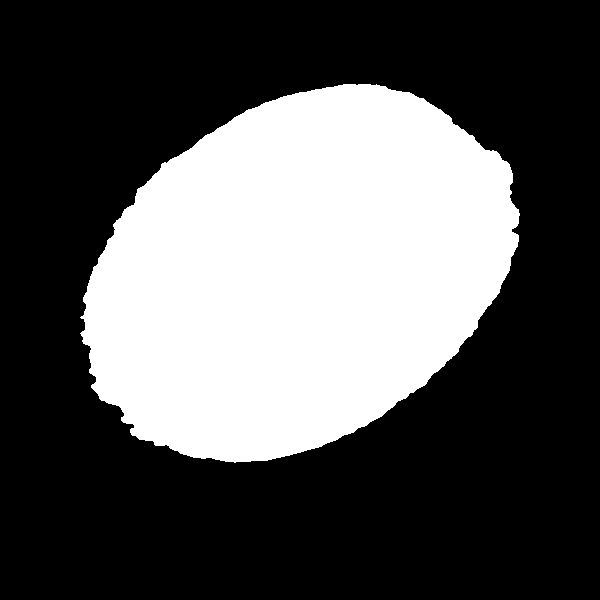
\includegraphics[width=.32\linewidth]{diff/m0_mask.png}
     }
     \hfill
    \subfloat[FPGA + DT segmentation\label{fma}]{%
       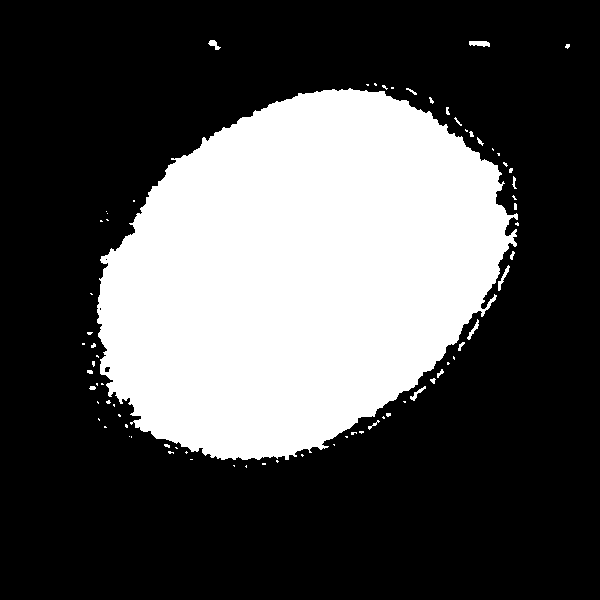
\includegraphics[width=.32\linewidth]{diff/m0_maskfpga.png}
     }
     \hfill
    \subfloat[Error\label{dma}]{%
       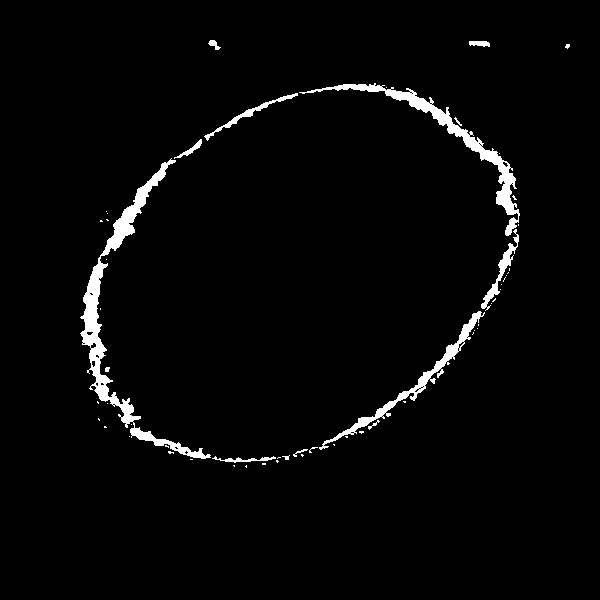
\includegraphics[width=.32\linewidth]{diff/m0_maskdif.png}
     }

    %\caption{Segmentation outputs.}
    \label{diffima}
    \end{figure}
    
  
\end{frame}



\begin{frame}
\frametitle{Thresholding algorithm comparison shifting}
    \begin{figure}[h]
    \centering
    \captionsetup[subfigure]{labelformat=empty}
    \subfloat[PC segmentation\label{oma}]{%
       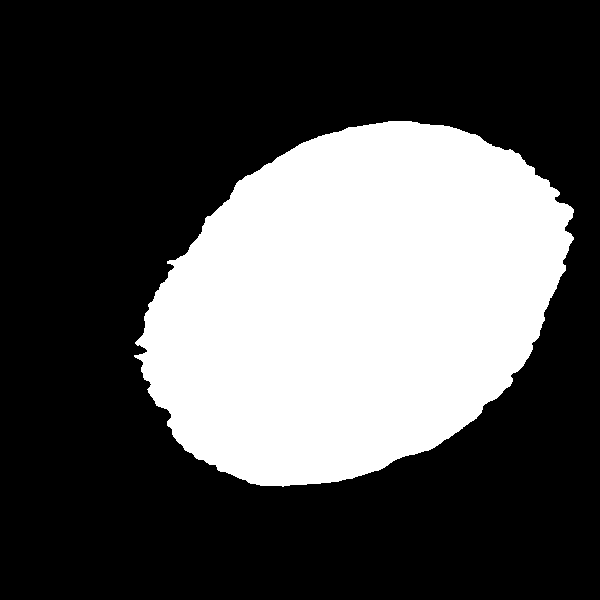
\includegraphics[width=.32\linewidth]{wrong/m45_mask.png}
     }
     \hfill
    \subfloat[FPGA + DT  segmentation\label{fma}]{%
       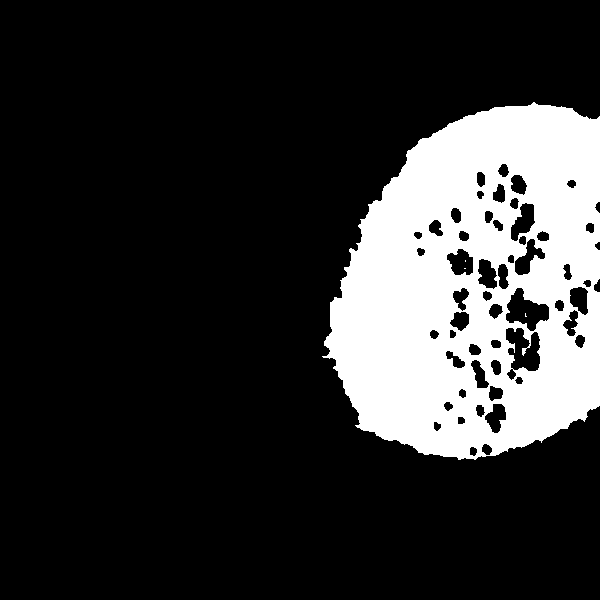
\includegraphics[width=.32\linewidth]{wrong/m45_maskfpga.png}
     }\hfill
    \subfloat[Error\label{dma}]{%
       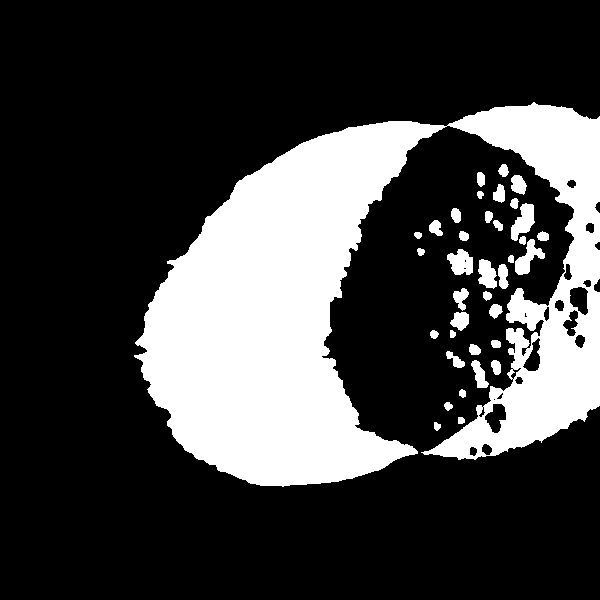
\includegraphics[width=.32\linewidth]{wrong/m45_maskdif.png}
     }
    %\caption{Sample of differential segmentation from shifted frame.}
    \label{wsample}
    \end{figure}
\end{frame}

\begin{frame}
\frametitle{Segmentation}


    \begin{table}[h]
\centering
\caption*{MODEL SEGMENTATION ACCURACY RESULTS}
%\resizebox{\linewidth}{!}{%
    \begin{tabular}{|c|c|c|c|}
    \hline
    Model &  Samples  & \% Range & Accuracy \\
    \hline
    M0 &  145 & 73.61\% - 96.46\%  & 84.54\%\\
    \hline
    M1 &  145 & 80.01\% - 99.02\% & 96.22\%\\
        \hline
    M2 &  155 & 87.77\% - 99.18\% & \textbf{97.10}\%\\
        \hline
    M3 &  153 & 88.22\% - 99.09\% & 96.64\%\\
        \hline
    M4 &  151 & 70.69\% - 98.76\% & 87.36\%\\
        \hline
    M5 &  138 & 64.81\% - 98.71\% & 94.14\%\\
        \hline
    
    \end{tabular}
%}
    \label{secomp}
\end{table}

$M2$ result as the best model, according to the feature relevance analysis. $M1$ and $M5$ got better results than they non-MOM complements. Morphologic Operations models get a better result  but is more important to get a model with the most important features.\\
Different number of sample since shifting in some cases.

\end{frame}

\begin{frame}
\frametitle{Model resource usage}
\begin{table}[ht]
\centering
%\caption*{}
%\resizebox{\linewidth}{!}{%
\begin{tabular}{|c|c|c|}
\hline


\textbf{Model}       & \textbf{Used Slices } & \textbf{Usel LUTs} \\ \hline
\textit{M0} & 5987 (3\%)  & 6012 (6\%) \\ \hline
\textit{M1} & \textbf{6110} (3\%)  & \textbf{6111} (6\%) \\ \hline
\textit{M2} & 5987 (3\%)  & 5899 (6\%) \\ \hline
\textit{M3} & 6110 (3\%)  & 5959 (6\%) \\ \hline
\textit{M4} & 5810 (3\%)  & 5377 (6\%) \\ \hline
\textit{M5} & 5988 (3\%)  & 5588 (6\%) \\ \hline
\end{tabular}
\label{res}
\end{table}

Almost all models uses same amount percent of the resources of the FPGA. 

\end{frame}

\begin{frame}
	\frametitle{Clasificación de color}
	
Naranjas analizadas: 549
\begin{itemize}
	\item Naranjas: 475
	\item Verdes: 74
\end{itemize}


Aciertos: 513
\begin{itemize}
	\item Naranjas: 445
	\item Verdes: 68
\end{itemize}


Presición: 93.44\%
\begin{itemize}
	\item Naranjas: 93.68\%
	\item Verdes: 91.89\%
\end{itemize}


	
\end{frame}



\begin{frame}
\frametitle{Conclusions and future work}

\begin{itemize}

\item The proposed decision-tree model: uses very few resources, another processing line can be processed in same device.

\item La clasificación por color es posible mediante modelos de árboles de decisión.

\item The proposed architecture results show that the system will be able to classify 5 ops by color and size. This represents 1 fruit-ton of classified fruits in approximately 18 minutes.
\end{itemize}

\end{frame}


\section{Acknowledgment}
\begin{frame}
\frametitle{Acknowledgment}
This work was supported by:

\begin{itemize}
\item CONACyT, Mexico, under research grant No. 933607
\item Electrónica y Automatización del Noreste S.A. de C.V. (EANSA)  and Red Tecnológica Tamaulipas (RedTam) for bringing equipment and machinery. \\

\end{itemize}



\end{frame}


% \begin{frame}[allowframebreaks]
% \frametitle{References}
% \insertBib
% 
% \end{frame}


\end{document}

